\chapter{Characters}

There are five major customization systems in Rise that all characters share.
In rough order of how much they affect your character's play style, they are your class archetypes, attributes, skills, insight points, and species.
At the GM's discretion, you may also have one or more feats, which can have a strong impact on your character's identity (see \pcref{Feats}).

This chapter explains those five fundamental elements.
If you plan on playing a premade character, the information in this chapter will still be useful so you can understand how your character works, but you can skip the Character Creation section at the end.
Some of the information in this chapter won't fully make sense until you've read future chapters.
You can either skim past terms you don't yet understand or look them up as you go along.

\section{Classes Overview}
    Each character has one of ten classes.
    Your class determines what your character's fundamental source of power is, and has a large impact on the play style of your character.
    Of course, any two members of the same class can be very different in both narrative style and mechanics based on the other choices they have made.
    Classes are intended as an aid to help give your character a cohesive identity, not a limitation on the possible character concepts you can fulfill.

    The ten classes are briefly summarized below.
    Each class has five archetypes, and any individual character chooses three of the five archetypes from their class.
    For full details about how each class works, see \pcref{Classes}.
    \begin{raggeditemize}
        \item Barbarians are primal warriors who draw power from their physical prowess and unfettered emotions.
        \item Clerics are divine spellcasters who draw power from their veneration of a single deity.
        \item Druids are nature spellcasters who draw power from their veneration of the natural world.
        \item Fighters are highly disciplined warriors who excel in physical combat of any kind.
        \item Monks are agile masters of ``ki'' who hone their personal abilities to strike down foes and perform supernatural feats.
        \item Paladins are divinely empowered warriors who exemplify a particular alignment.
        \item Rangers are skilled hunters who bridge the divide between nature and civilization.
        \item Rogues are exceptionally skillful characters known for their ability to strike at their foe's weak points in combat.
        \item Sorcerers are arcane spellcasters who draw power from their inherently magical nature.
        \item Warlocks are pact spellcasters who draw their power from a sinister deal made with infernal creatures.
        \item Wizards are arcane spellcasters who study magic to unlock its powerful secrets.
    \end{raggeditemize}

\section{Attributes}\label{Attributes}

    Each character has six \glossterm{attributes}: Strength (Str), Dexterity (Dex), Constitution (Con), Intelligence (Int), Perception (Per), and Willpower (Wil).
    Each attribute represents a character's raw talent in that area.

    A 0 in an attribute represents average human capacity.
    That doesn't mean that every commoner has a 0 in every attribute; not everyone is average, after all.

    \subsection{Strength (Str)}\label{Strength}
        {
            Strength measures your muscle and physical power.
            Characters with a high Strength tend to have strong offensive capabilities with nonmagical abilities, and prefer wearing heavier armor.
            It has the following effects:
            \begin{raggeditemize}
                \item Strength determines how much you can carry (see \tref{Weight Limits by Strength}).
                    You generally need a Strength of at least 1 to wear heavy body armor.
                \item You add half your Strength in \glossterm{dice increments} to your damage and healing with \glossterm{mundane} abilities (see \pcref{Dice Bonuses From Attributes}).
                \item If your Strength is positive, you reduce your \glossterm{encumbrance} from \glossterm{armor} by an amount equal to your Strength (see \pcref{Encumbrance}).
                \item You add your Strength to Strength-based \glossterm{skills}: Climb, Jump, and Swim (see \pcref{Skills}).
            \end{raggeditemize}
        }

    \subsection{Dexterity (Dex)}\label{Dexterity}
        {
            Dexterity measures your hand-eye coordination, agility, and reflexes.
            Characters with a high Dexterity tend to have strong defensive capabilities, and prefer wearing lighter armor.
            It has the following effects:
            \begin{raggeditemize}
                \item You add your Dexterity to your Reflex defense.
                \item You add your Dexterity to your Armor defense.
                    This bonus can be reduced if you use medium or heavy armor (see \tref{Armor and Shields}).
                \item You add your Dexterity to Dexterity-based \glossterm{skills}: Balance, Flexibility, Ride, Sleight of Hand, and Stealth (see \pcref{Skills}).
            \end{raggeditemize}
        }

    \subsection{Constitution (Con)}\label{Constitution}
        {
            Constitution represents your health and stamina.
            Characters with a high Constitution tend to have strong defensive capabilities.
            It has the following effects:
            \begin{raggeditemize}
                \item You add your Constitution to your level for the purpose of determining your \glossterm{hit points} and \glossterm{damage resistance} (see \pcref{Hit Points}, and \pcref{Damage Resistance}).
                \item You add your Constitution to your \glossterm{fatigue tolerance} (see \pcref{Fatigue}).
                \item You add your Constitution to your Fortitude defense.
                \item You add your Constitution to the Constitution-based \glossterm{skill}: Endurance (see \pcref{Skills}).
            \end{raggeditemize}
        }

    \subsection{Intelligence (Int)}\label{Intelligence}
        {
            Intelligence represents how well you learn and reason.
            Characters with a high Intelligence tend to have more options and special abilities.
            It has the following effects:

            \begin{raggeditemize}
                \item If your Intelligence is positive, you become \glossterm{trained} in a number of skills equal to your Intelligence (see \pcref{Trained Skills}).
                \item You add your Intelligence to the number of \glossterm{insight points} you gain (see \pcref{Insight Points}).
                \item You add your Intelligence to Intelligence-based \glossterm{skills}: Craft, Deduction, Disguise, Knowledge, Linguistics, and Medicine (see \pcref{Skills}).
            \end{raggeditemize}

            \par Non-sentient creatures like animals have an Intelligence of \minus6 or lower.
            Sentient creatures have an Intelligence of at least \minus5.
        }

    \subsection{Perception (Per)}\label{Perception}
        {
            Perception describes your ability to observe and be aware of your surroundings.
            Characters with a high Perception tend to have strong offensive capabilities.
            It has the following effects:
            \begin{raggeditemize}
                \item You add half your Perception to your \glossterm{accuracy} with all attacks (see \pcref{Accuracy}).
                \item You add your Perception to Perception-based \glossterm{skills}: Awareness, Creature Handling, Social Insight, and Survival (see \pcref{Skills}).
            \end{raggeditemize}
        }

    \subsection{Willpower (Wil)}\label{Willpower}
        {
            Willpower represents your ability to endure mental hardships.
            Characters with a high Willpower tend to be better at attacking with and defending against magical abilities.
            It has the following effects:
            \begin{raggeditemize}
                \item You add half your Willpower in \glossterm{dice increments} to your damage and healing with \glossterm{magical} abilities (see \pcref{Dice Bonuses From Attributes}).
                \item You add half your Willpower to your \glossterm{fatigue tolerance} (see \pcref{Fatigue}).
                \item You add your Willpower to your Mental defense.
            \end{raggeditemize}
        }

\section{Skills Overview}
    Skills represent the myriad of talents that people can have, such as cooking or swimming.
    Each character is trained in a certain number of skills.
    If you are trained in a skill, you have a higher likelihood of succeeding when you try to use it.
    The number of skills you are trained in is mostly determined by your class and Intelligence.

    The twenty-six skills are summarized below.
    For full details about how each skill works, see \pcref{Skills}.

    \begin{raggeditemize}
        \item The Awareness skill represents your ability to observe things which you might otherwise fail to notice.
        \item The Balance skill represents your ability to maintain your balance and poise in difficult circumstances.
        \item The Climb skill represents your ability to climb obstacles.
        \item The Craft skills represent your ability to construct objects from raw materials.
        \item The Creature Handling skill represents your ability to influence non-sapient creatures.
        \item The Deception skill represents your ability to lie or otherwise mislead people without being caught.
        \item The Deduction skill represents your ability to make logical deductions based on evidence.
        \item The Devices skill represents your ability to to manipulate mechanical devices such as locks, traps, and other contraptions.
        \item The Disguise skill represents your ability to create disguises to conceal the appearance of creatures or objects.
        \item The Endurance skill represents your ability to persevere through physical trials.
        \item The Flexibility skill represents your ability to escape bindings and move through small areas by contorting your body.
        \item The Intimidate skill represents your ability to intimidate and coerce people into doing what you want.
        \item The Jump skill represents your ability to jump.
        \item The Knowledge skills represent your understanding of particular aspects of the world.
        \item The Linguistics skill represents your mastery of spoken and written languages.
        \item The Medicine skill represents your practical understanding of how to tend to the wounds of living creatures.
        \item The Perform skills represent your ability to create particular forms of entertainment.
        \item The Persuasion skill represents your ability to convince people to think what you want them to.
        \item The Profession skills represent your practical understanding of a particular profession.
        \item The Ride skill represents your ability to ride and control horses and other mounts.
        \item The Sleight of Hand skill represents your ability to pick pockets, palm objects, and perform other feats of legerdemain.
        \item The Social Insight skill represents your ability to read body language and emotion.
        \item The Stealth skill represents your ability to escape detection while moving or taking large-scale actions.
        \item The Survival skill represents your ability to take care of yourself and others in the wilderness, including the ability to follow tracks.
        \item The Swim skill represents your ability to swim.
    \end{raggeditemize}

\section{Insight Points}\label{Insight Points}
    You can spend \glossterm{insight points} to gain new special abilities.
    Your \glossterm{class} gives you a certain number of insight points, and you gain a bonus (or penalty) to that number of insight points equal to your Intelligence.
    Some abilities can also grant insight points.
    
    You can spend two \glossterm{insight points} to become a \glossterm{multiclass} character (see \pcref{Multiclass Characters}).
    In addition, every class has at least one way to spend \glossterm{insight points} to learn additional abilities.
    These options are listed below.
    \begin{itemize}
        \item Barbarian: Combat styles and maneuvers
        \item Cleric: Metamagic, mystic spheres, and spells
        \item Druid: Metamagic, mystic spheres, spells, and wild aspects
        \item Fighter: Battle tactics, combat styles, and maneuvers
        \item Fighter: Combat styles, ki manifestations, and maneuvers
        \item Paladin: Mystic spheres and spells
        \item Ranger: Combat styles, hunting styles, and maneuvers
        \item Rogue: Bardic performances, combat styles, maneuvers, and trained skills
        \item Sorcerer: Metamagic, mystic spheres, and spells
        \item Warlock: Metamagic, mystic spheres, and spells
        \item Wizard: Metamagic, mystic spheres, and spells
    \end{itemize}

\section{Species}\label{Species}
    Each character has a species.
    There are seven common species described below.
    At the GM's discretion, you may be able to play a character with a more unusual species (see \pcref{Uncommon Species}).

    \subsection{Humans}
        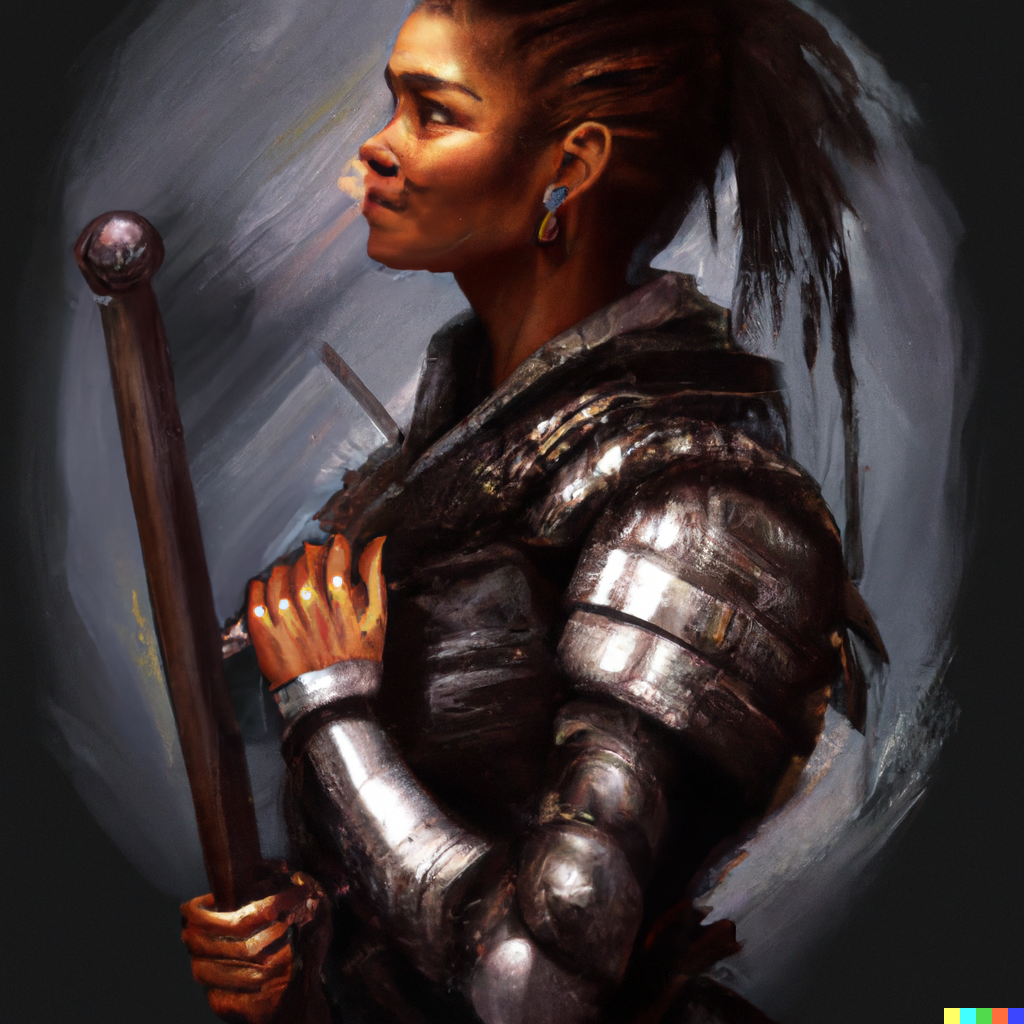
\includegraphics[width=\columnwidth]{characters/human}

        Humans are the most common and least rigidly defined of all Rise species.
        They are not the smartest, the strongest, or the most durable of the civilized races.
        They have no supernatural senses or impossible talents; anything a human can do, a member of another species could do at least as well.
        Despite their limitations, humans are practically universal, and their civilizations are the most powerful and numerous of all.

        The success of humanity comes from one core strength: their adaptability, both individually and as a whole.
        Individual humans can learn new skills with surprising ease compared to other species, and they often have a breadth of talent that few can rival.
        The relatively short human lifespan prevents their society from stagnating under the guidance of elders whose wisdom is now hundreds of years out of date.
        When radical changes sweep the world, humans can adapt where other species would founder.

        \parhead{Size} Medium.
        \parhead{Attributes} No change.
        \parhead{Special Abilities}
        \begin{raggeditemize}
            \itemhead{Flexible} Humans gain an additional \glossterm{insight point}.
                Insight points can be spent to learn new special abilities (see \pcref{Insight Points}).
            \itemhead{Skilled} Humans gain an additional \glossterm{trained skill} (see \pcref{Skills}).
        \end{raggeditemize}
        \parhead{Automatic Language} Common, any two \glossterm{common languages} or one \glossterm{rare language} (see \pcref{Communication and Languages}).

    \subsection{Dwarves}
        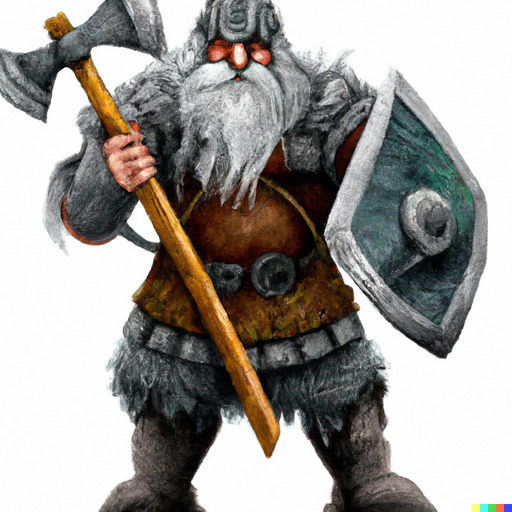
\includegraphics[width=\columnwidth]{characters/dwarf}

        Dwarves are short, stout, and sturdy.
        It has been said that the first dwarf was carved from stone, and the similarities have been noted by many.
        All dwarves naturally have beards, and the vast majority keep them long and elegantly maintained.

        Most dwarves live underground in mining communities.
        These communities can grow to massive size, and dwarven kings can rule vast underground cities.
        The dwarven fascination with strong drink is legendary, though somewhat misleading.
        Their natural resilience means they need stronger drinks to even notice the effects, so other species tend to gain an exaggerated impression of dwarven drunkenness when they try to drink dwarven ale.

        \parhead{Size} Medium.
        \parhead{Attributes} \plus1 Constitution, \minus1 Dexterity.
        \parhead{Special Abilities}
        \begin{raggeditemize}
            \itemhead{Darkvision} Dwarves have \trait{darkvision} with a 60 foot range, allowing them to see in complete darkness (see \pcref{Darkvision}).
            \itemhead{Depth Sense} Dwarves can intuitively sense their approximate depth underground as naturally as a human can sense which way is up.
            \itemhead{Earthen Crafting} Dwarves gain a \plus2 bonus to the Craft (metal) and Craft (stone) skills.
            \itemhead{Enduring} Dwarves gain a \plus1 bonus to their \glossterm{fatigue tolerance}.
            \itemhead{Slow and Steady} Dwarves have a \minus10 foot penalty to their speed with all \glossterm{movement modes}.
                However, wearing heavy \glossterm{body armor} does not reduce a dwarf's speed (see \pcref{Armor Usage Classes}).
                In addition, a dwarf's land speed cannot be reduced below 10 feet.
            \itemhead{Stable} Dwarves reduce the distance they are moved by unwilling \glossterm{knockback} and \glossterm{push} effects by 20 feet.
        \end{raggeditemize}
        \parhead{Automatic Languages} Common, Dwarven, any one \glossterm{common language} (see \tref{Common Languages}).

    \subsection{Elves}
        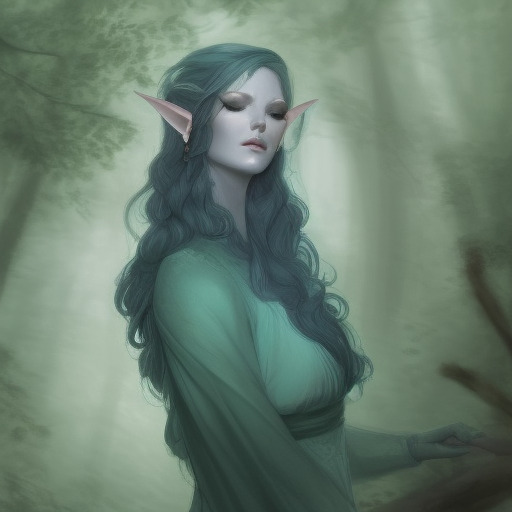
\includegraphics[width=\columnwidth]{characters/elf}

        Elves are tall, lithe, and graceful.
        They tend to have an air of confidence at all times, and even their mistakes seem intentional.
        Elves have the longest lifespan of any civilized species, and even comparatively young elves carry a weight of experience that can be daunting for non-elves.

        For millenia, elves were the most powerful civilization above ground, while dwarves claimed the underground.
        More recently, humans have usurped elves as the most powerful civilization above ground, while dwarves have kept their claim.
        This history, combined with their natural differences, has created an ancient rivalry between elves and dwarves that sometimes manifests as outright hatred.

        \parhead{Size} Medium.
        \parhead{Attributes} \minus1 Constitution, either \plus1 Dexterity or \plus1 Perception.
        \parhead{Special Abilities}
        \begin{raggeditemize}
            \itemhead{Elven Serenity} Elves gain a \plus1 bonus to Mental defense.
            \itemhead{Keen Senses} Elves gain a \plus2 bonus to the Awareness skill (see \pcref{Awareness}).
            \itemhead{Low-light Vision} Elves have \trait{low-light vision}, allowing them to see clearly in \glossterm{shadowy illumination} (see \pcref{Low-light Vision}).
            \itemhead{Sure-Footed} Elves gain a \plus2 bonus to the Balance skill (see \pcref{Balance}).
            \itemhead{Trance} Elves do not sleep, and are immune to \glossterm{magical} effects that would cause them to sleep.
                Instead of sleeping, elves can trance for 4 hours.
                An elf in trance may make Perception-based checks at a \minus5 penalty.
                Elves must still avoid strenuous activity for 8 hours to heal and gain other benefits of taking a \glossterm{long rest}.
        \end{raggeditemize}
        \parhead{Automatic Languages} Common, Elven, any one \glossterm{common language} (see \tref{Common Languages}).

    \subsection{Gnomes}
        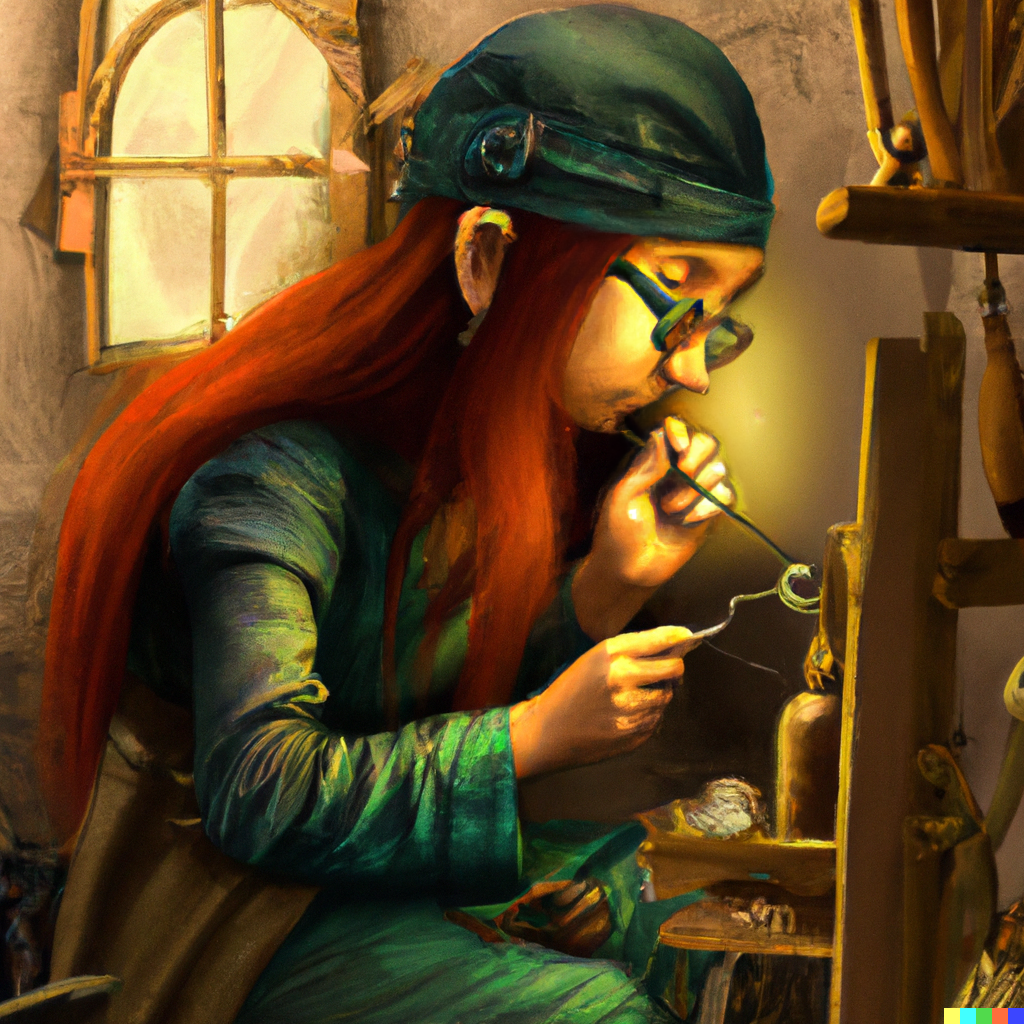
\includegraphics[width=\columnwidth]{characters/gnome}

        Gnomes are the smallest, most magical, and most short-lived of the civilized species.
        Their large eyes and heads give even adult gnomes almost child-like proportions.
        Fae blood runs in the blood of all gnomes, and gnome societies have many traditions and rituals that seem superstitious to outsiders.
        However, these rituals have a purpose, and gnomes understand that failing to appease the hidden powers in the world can have dangerous consequences.

        Most gnomes live in forests, but they can be found in remote areas all over the world.
        Gnomish settlements are almost always overseen by minor fae, such as dryads, who protect the settlement.
        In many cases, the settlements were originally built around a site of mystic power, though some settlements have outlived their original protectors.

        \parhead{Size} Medium.
        \parhead{Attributes} \minus1 Strength, either \plus1 Constitution or \plus1 Intelligence.
        \parhead{Special Abilities}
        \begin{raggeditemize}
            \itemhead{Fae Light}[Magical] A gnome can use the \textit{fae light} ability as a standard action.
                \begin{activeability}{Fae Light}
                    \rankline
                    A Tiny glowing orb appears at a location within \rngmed range.
                    It sheds pale, \glossterm{bright illumination} in a \areasmall radius, and \glossterm{shadowy illumination} in a \areamed radius.
                    The orb is intangible, and cannot be moved once placed.

                    This ability lasts until you use it again or until you \glossterm{dismiss} it as a free action.
                \end{activeability}
            \itemhead{Magic Affinity} Gnomes gain an additional \glossterm{insight point}.
                They can only spend this insight point to learn \glossterm{magical} abilities, such as spells.
            \itemhead{Short Stature} Gnomes gain a \plus2 bonus to the Stealth skill.
            \itemhead{Tinkerer} Gnomes gain a \plus2 bonus to two Craft skills of their choice (see \pcref{Craft}).
        \end{raggeditemize}
        \parhead{Automatic Languages} Common, Gnome, either Sylvan or any one \glossterm{common language} (see \tref{Common Languages}).

    \subsection{Half-Elves}\label{Half-Elves}
        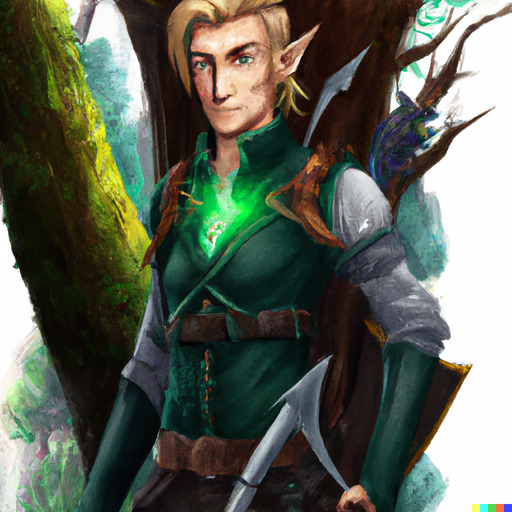
\includegraphics[width=\columnwidth]{characters/halfelf}

        Half-elves carry both human and elven heritage.
        They are caught between two worlds, with neither the unconscious grace of elves nor the limitless adaptability of humans.
        However, they have their own unique forms of versatility based on their understanding of both worlds.

        \parhead{Size} Medium.
        \parhead{Attributes} No change.
        \parhead{Special Abilities}
        \begin{raggeditemize}
            \itemhead{Diplomatic} Half-elves gain a \plus2 bonus to the Persuasion skill.
            \itemhead{Low-light Vision} Half-elves have \trait{low-light vision}, allowing them to see clearly in \glossterm{shadowy illumination} (see \pcref{Low-light Vision}).
            \itemhead{Versatile} Half-elves only need to spend one \glossterm{insight point} to gain access to an additional class (see \pcref{Multiclass Characters}).
        \end{raggeditemize}
        \parhead{Automatic Language} Common, Elven, any two \glossterm{common languages} or one \glossterm{rare language} (see \pcref{Communication and Languages}).

    \subsection{Half-Orcs}
        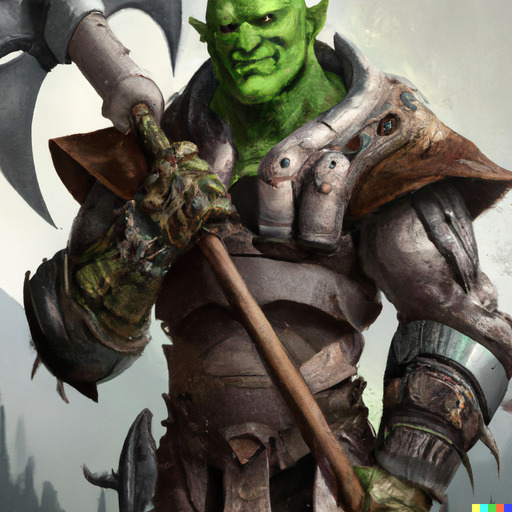
\includegraphics[width=\columnwidth]{characters/halforc}

        Half-orcs carry both human and orcish heritage.
        They have much of the brute strength of orcs, but tempered by human adaptability.

        \parhead{Size} Medium.
        \parhead{Attributes} \plus1 Strength, \minus1 Intelligence.
        \parhead{Special Abilities}
        \begin{raggeditemize}
            \itemhead{Darkvision} Half-orcs have \trait{darkvision} with a 60 foot range, allowing them to see in complete darkness (see \pcref{Darkvision}).
            \itemhead{Intimidating} Half-orcs gain a \plus2 bonus to the Intimidate skill (see \pcref{Intimidate}).
            \itemhead{Physical Instincts} Half-orcs gain an additional \glossterm{insight point}.
                They can only spend this insight point to learn \glossterm{mundane} abilities, such as combat styles and maneuvers.
        \end{raggeditemize}
        \parhead{Automatic Languages} Common, Orcish.

    \subsection{Halflings}
        
\includegraphics[width=\columnwidth]{characters/halfling}

        Halflings stand at about half the height of a human, but have generally human-like proportions.
        They tend to be plucky, adventurous, and outgoing.
        Of all species, halflings have the fewest halfling-only communities.
        Instead, halfling groups tend to live in the gaps between the ``big people'', especially in large cities.

        \parhead{Size} Medium.
        \parhead{Attributes} \minus1 Strength, either \plus1 Dexterity or \plus1 Willpower.
        \parhead{Special Abilities}
        \begin{raggeditemize}
            \itemhead{Nimble Combatant} Halflings gain a \plus1 bonus to Reflex defense.
            \itemhead{Short Stature} Halflings gain a \plus2 bonus to the Stealth skill.
            \itemhead{Stout-Hearted} Halflings gain a \plus1 bonus to Mental defense.
            \itemhead{Sure-Footed} Halflings gain a \plus2 bonus to the Balance skill (see \pcref{Balance}).
        \end{raggeditemize}
        \parhead{Automatic Languages} Common, Halfling, any one \glossterm{common language} (see \tref{Common Languages}).

\section{Alignment}\label{Alignment}
    A creature's general moral and personal attitudes are represented by its alignment: lawful good, neutral good, chaotic good, lawful neutral, neutral, chaotic neutral, lawful evil, neutral evil, or chaotic evil.

    Alignment is a tool for developing your identity.
    It is not a straitjacket for restricting your actions.
    Each alignment represents a broad range of personality types or personal philosophies, so two characters of the same alignment can still be quite different from each other.
    In addition, few people are completely consistent.

    \subsection{Good vs. Evil}
        The ancient battle between good and evil takes many forms, and distinguishing good from evil is a deeply complex task.
        For the purposes of Rise, good and evil are strictly defined according to selfishness vs. altruism.
        The actions of good characters may at times be morally reprehensible, and the actions of evil characters may seem to be virtuous.
        However, this narrow definition of good and evil avoids the complexities of defining a more robust moral system while preserving the fundamental conflict between good and evil.

        \parhead{Good} Good characters are altruistic.
        They take other creatures into account when making decisions, and actively try to help or improve others around them.
        Good characters may have significant disagreements about what actions are best, but they consistently prioritize the good of others or the ``greater good'' over their own desires.
        Different good characters may also have different perspectives on who they should take into account when making decisions.
        For example, some good characters actively work to protect animals and plants, while others only care about sapient creatures.

        Sometimes, altruistic characters can commit reprehensible actions out of necessity or because they believe that a greater good is being served.
        As long as their motivation is selfless, those characters are still considered to be ``good'' from the perspective of Rise's alignment system, which does not attempt to model all of the complexities of real-world morality.

        \parhead{Evil} Evil characters are selfish.
        They consistently prioritize their own desires and needs over the desires of others, even their allies or friends.
        Evil characters may take actions that help others and can even work effectively as a team, but their ultimate motivation is to help themselves or make themselves feel better, not to help others.

        \parhead{Neutral} Characters that are neutral between good and evil are neither consistently altruistic nor consistently selfish.
        Most neutral characters behave altruistically in some ways and selfishly in other ways -- either at different times, or about different aspects of life.
        They often have strong bonds to particular individuals who they care about selflessly, but are not altruistic in a general sense.
        Non-sapient beings such as animals are neutral rather than good or evil.

    \subsection{Law vs. Chaos}
        \parhead{Law} Lawful characters value consistency.
        They obey rules that guide their actions.
        Some lawful characters draw their rules from external forces, such as serving a particular master or following the legal laws of the land.
        Other lawful characters follow rules they make for themselves.

        \parhead{Chaos} Chaotic characters value flexibility and freedom.
        They make decisions based on what they think or feel at the time, even if it is inconsistent with their previous statements or actions.

        \parhead{Neutral} Characters that are neutral between law and chaos are neither exceptionally consistent nor exceptionally inconsistent.
        They tend to be generally consistent but may change their minds under the right circumstances.
        Non-sapient beings such as animals are neutral rather than lawful or chaotic.

\section{Personal Appearance}
    \begin{dtable!*}
        \lcaption{Typical Ages}
        \begin{dtabularx}{\textwidth}{l *{5}{>{\ccol}X}}
            \tb{Species} & \tb{Adulthood} & \tb{Middle Age} & \tb{Old}  & \tb{Venerable} & \tb{Maximum Age} \tableheaderrule
            Human        & 15 years       & 35 years        & 55 years  & 70 years       & \plus4d10 years \\
            Dwarf        & 40 years       & 125 years       & 190 years & 250 years      & \plus2d\% years \\
            Elf          & 110 years      & 175 years       & 250 years & 350 years      & \plus4d\% years \\
            Gnome        & 10 years       & 25 years        & 40 years  & 55 years       & \plus1d10 years \\
            Half-elf     & 20 years       & 60 years        & 90 years  & 125 years      & \plus6d10 years \\
            Half-orc     & 14 years       & 30 years        & 45 years  & 60 years       & \plus2d10 years \\
            Halfling     & 20 years       & 50 years        & 75 years  & 100 years      & \plus1d\% years \\
        \end{dtabularx}
    \end{dtable!*}

    \begin{dtable}
        \lcaption{Typical Height and Weight}
        \begin{dtabularx}{\columnwidth}{l *{2}{>{\lcol}X}}
            \tb{Species} & \tb{Average Height} & \tb{Average Weight} \tableheaderrule
            Human        & 5' 5''              & 150 lb. \\
            Dwarf        & 4' 2''              & 160 lb. \\
            Elf          & 5' 0''              & 110 lb. \\
            Gnome        & 3' 4''              & 50 lb.  \\
            Half-elf     & 5' 2''              & 130 lb. \\
            Half-orc     & 5' 10''             & 200 lb. \\
        \end{dtabularx}
    \end{dtable}

    \subsection{Age}
        The typical age for each species is listed in \trefnp{Typical Ages}.
        If you are old, you take a \minus2 penalty to \glossterm{checks} based on Strength, Dexterity, Constitution, and Perception.
        However, you gain a \plus2 bonus to \glossterm{checks} based on Intelligence and Willpower.
        If you are venerable, these modifiers change to \minus4 and \plus4 respectively.
        In general, player characters should not start as old or venerable age, but the GM can always allow it for specific campaigns if they want.

        When you reach venerable age, the GM secretly rolls your maximum age, which is the number from the Venerable column on \trefnp{Typical Ages} plus the result of the dice roll indicated on the Maximum Age column on that table.
        They record the result.
        If you reach your maximum age, you die of old age at some time during the following year.

        The maximum ages are for player characters. Most people in the world at large die from pestilence, accidents, infections, or violence before getting to venerable age.

    \subsection{Height and Weight}
        The typical height and weight for each species is listed in \tref{Typical Height and Weight}.
        The average man from each species is slightly taller and heavier than the average woman, but this is not a restriction for player characters.

\section{Character Creation}\label{Character Creation}

    Creating a charcter involves a mixture of thematic and mechanical decisions that will work together to create a fun character that is rewarding to play.
    As mentioned earlier in this chapter, there are four core systems for customizing your character's mechanics: class, attributes, skills, and species.
    In addition, there are five core thematic considerations when creating a character: concept, personality, motivation, background, and appearance.

    These decisions are described below in a order that makes sense for many characters, and full details for each decision are given after this initial list.
    It is essentially a sandwich, with narrative decisions wrapped around a central core of your character's mechanical components.
    However, you can make several of these decisions in any order, and you may find it easier to create a character in a different way.
    The only real limitation is that your skills must be the last mechanical choice you make, since they are strongly affected by all of your other choices.

    \begin{enumerate}
        \item Character concept: Describe your character with a short, simple phrase that captures their essence.
        \item Motivation and goal: Describe what your character wants.
        \item Alignment: Describe your character's moral compass.

        \item Species: Define your character's species.
        \item Attributes: Define your character's fundamental physical and mental potential.
        \item Class archetypes: Define your character's source of power.
        \item Insight points: Learn new abilities.
        \item Skills: Define your character's areas of non-combat expertise.

        \item Personality: Describe how your character acts and reacts to the world.
        \item Background: Describe what made your character become who they are now.
        \item Appearance: Describe what your character looks like.
        \item Name: Choose a name.
    \end{enumerate}

    \subsection{Step 1: Character Concept}

        Fundamentally, who is your character?
        You should think of a short phrase that describes the core concept behind the character you will create.
        It's best to think in broad strokes when creating a character concept.
        Your concept should be more than just a factual description of your species or what you do.
        It should be something that makes you memorable.
        Some sample character concepts are given below for inspiration.

        \begin{raggeditemize}
            \item Pragmatic wanderer
            \item Artistic pixie
            \item Mushroom-obsessed hermit
            \item Bumbling do-gooder
            \item Dim-witted bodyguard
            \item Cowardly storyteller
            \item Bear-barian
            \item Parsimonious law enforcer
            \item Peaceful naturalist
            \item Trigger-happy pyromaniac
            \item Heroic, simple-minded warrior
            \item Friendly necromancer
            \item Chaotic speed demon
            \item Pompous ex-noble
            \item Sarcastic mercenary
            \item Battle-scarred priest
            \item Ambitious arcane prodigy
            \item Charismatic musician
            \item Aloof scholar
            \item Blunt-spoken warrior
            \item Crazed prophet
            \item Polite warrior
            \item World-weary pirate
            \item Devout cultist
            \item Con artist with a heart of gold
        \end{raggeditemize}

    \subsection{Step 2: Motivation and Goal}
        Why does your character put in all of the effort that adventuring requires?
        They probably have a goal that they are trying to achieve, or an ideal that they are trying to embody.
        Writing down a specific goal or ideal can be helpful as an anchor point when defining the character.

    \subsection{Step 3: Alignment}
        Your character's alignment reflects their moral character: are they more inclined to good or evil, and to chaos or order?
        Alignments are described in more detail at \pcref{Alignment}.

    \subsection{Step 4: Species}
        It's often convenient to make your species your first mechanically relevant choice.
        Your species can have a strong effect on your personality and narrative, but it has a relatively small effect on your character's play style.
        It's also easier to know your species before you choose your attributes, since your species can slightly modify your attributes.

        Choose one of the seven common species options, or talk with your GM about choosing an uncommon species (see \pcref{Uncommon Species}).
        Record any specific abilities the species gives you on your character sheet, but if this is your first mechanical choice, you won't be able to finalize any of your statistics yet.
        You should also choose the languages that you can speak, since that is influenced by your species (see \pcref{Communication and Languages}).

    \subsection{Step 5: Attributes}
        Your attributes are a good option for your second mechanically relevant choice.
        They have a large impact on your character's strengths and weaknesses, so it's useful to know them as soon as possible.
        They're also much easier to understand and finalize than your class archetypes.

        There are two common ways for you to determine your attribute scores: using a predefined set of scores, or using a point buy system.
        Once you have chosen your attributes and applied your species modifer to attributes (if any), you should record in your character sheets the various effects that your attributes have on your statistics.

        \subsubsection{Predefined Attribute Scores}
            This is the simplest method.
            Simply take the following set of attribute scores and distribute them as you choose among your attributes:

            % 5 + 3 + 3 + 3 + 1 = 15
            3, 2, 2, 2, 1, 0

            This set of attribute scores is called the ``elite array''.
            For more extreme characters, you may use the ``savant array'':

            % 8 + 3 + 3 + 1 = 15
            4, 2, 2, 1, 0, 0.

            Finally, for more well-rounded characters, you may use the ``balanced array'':

            % 3 + 3 + 3 + 3 + 3 = 15
            2, 2, 2, 2, 2, 0

        \subsubsection{Point Buy}
            With this method, you can fully control your attribute scores to precisely match what you want to be able to do.
            All your attribute scores start at 0.
            You get 15 points to distribute among your attributes.
            Attributes can be bought according to the costs on \trefnp{Attribute Score Point Costs}.
            The listed cost is the total cost required to gain the listed attribute.

            \begin{dtable}
                \tablebookmark{Attribute Point Costs}{attributepoints}
                \lcaption{Attribute Point Costs}
                \begin{dtabularx}{\columnwidth}{X X}
                    \tb{Attribute} & \tb{Cumulative Point Cost} \tableheaderrule
                    0              & 0                          \\
                    1              & 1                          \\
                    2              & 3                          \\
                    3              & 5                          \\
                    4              & 8                          \\
                \end{dtabularx}
            \end{dtable}

        \subsubsection{Attribute Penalties}\label{Attribute Penalties}
            You can voluntarily take penalties to your attributes.
            If you reduce an attribute to a total of \minus1, you become \glossterm{trained} in an additional skill (see \pcref{Trained Skills}).
            If you reduce an attribute to a total of \minus2, you instead gain an additional \glossterm{insight point} (see \pcref{Insight Points}).
            You cannot gain these benefits from reducing more than two attributes below 0 in this way.

    \subsection{Step 6: Class and Class Archetypes}
        This is the most complicated choice you have to make for your character.
        It requires the most reading in the Classes chapter to understand what your options are and which classes and class archetypes are interesting to you.
        Class details can be found in \pcref{Classes}.

        You should choose one of the ten classes, and then any one of the five archetypes within that class.
        You gain the rank 1 ability from that archetype.
        You should also choose the \glossterm{weapon groups} that you have access to, since that is influenced by your class (see \pcref{Weapon Groups}).

        When you reach levels 2 and 3, you'll choose new archetypes from the same class, becoming rank 1 in each of those archetypes as well.
        After that, you won't gain any more new archetypes when you gain levels.
        Instead, you'll just increase your rank in the three archetypes you already have.

        If you are particularly adventurous, this is also when you should choose if you want to be a multiclass character.
        Multiclass characters can gain access to archetypes from multiple classes.
        This does not increase the number of archetypes you know, so it does not directly increase your power.
        However, multiclass characters can be more specialized or more versatile than single-class characters, and can represent unusual character concepts.
        For details, see \pcref{Multiclass Characters}.

    \subsection{Step 7: Insight Points}
        Once you have chosen your class archetypes, attributes, and species, you know how many insight points you have, and can choose how to spend them.
        Don't forget to record on your character sheet how you spent each insight point.
        Otherwise, you might get confused later about why you have more spells known than you normally would.

        In some circumstances, you might want to delay spending your insight points until you are higher level.
        For example, a fighter/sorcerer multiclass character who wants to have both spells and maneuvers can't have access to both spells and maneuvers at level 1, so they wouldn't be able to spend insight points on both spells and maneuvers.
        You aren't forced to spend all of your insight points, so you can save them up for later.
        You can also talk to your GM about spending them at level 1 and then retraining those insight points once you are higher level.

    \subsection{Step 8: Skills}
        You should choose which skills you have \glossterm{trained} (see \pcref{Skills}).
        Your \glossterm{class} gives you a certain number of trained skills from among the \glossterm{class skills} for that class.
        The class skills for each class are summarized in \tref{Class Skills}.

        There are other ways to become trained in skills that are not part of your class.
        If your Intelligence is positive, you gain additional trained skills equal to your Intelligence.
        You can also spend \glossterm{insight points} to gain one trained skill per insight point (see \pcref{Insight Points}).
        Some abilities can grant additional trained skills.

        If you are untrained in a skill, your bonus with that skill is equal to half of its associated attribute (if any).
        If you are trained in a skill, your bonus with that skill is equal to 3 \add the higher of its associated attribute (if any) and half your level.
        Many abilities can increase or decrease your bonus with particular skills.

        The number of skills you can have trained, and which skills those are, depend on every preceding step, so it's a good place to finish.

        Sometimes, you might have more trained skills than you know what to do with, especially if you are still figuring out the details of your character concept.
        You aren't forced to decide all of your trained skills at level 1, so you can save them up and choose more trained skills when you level up.
        You can also talk to your GM about letting you decide your trained skills on the fly during the first game session or two based on what actions you take during the session.
        This can be a fun way to figure out what your character's personality is through the process of playing them.

    \subsection{Step 9: Starting Equipment}
        When you create a character, they can start with some basic items.
        Items have \glossterm{item ranks} that indicate the approximate rank that characters can reasonably get access to them.
        Typically, you can start with a single rank 1 item, up to three rank 0 items, and a standard adventuring kit.
        Individual campaigns or character backstories may significantly change what starting equipment is available, so check with your GM.

    \subsection{Step 10: Personality}

        How does your character behave?
        You should decide, in broad terms, what your character's personality is.
        This will change over time, especially as you start playing the character in the game, so you don't need to define everything perfectly.
        However, having a general sense of how your character behaves is helpful.

        For most games, it's important to have a personality that can tolerate working with others in a group.
        A character that is excessively aloof, moody, or obnoxious can make the game more difficult to enjoy for everyone.
        Likewise, a character who tries to speak for everyone or who repeatedly steals the spotlight from others can be frustrating to work with.
        You should figure out the right balance with your fellow players and your GM.\@

    \subsection{Step 11: Background}
        What happened in their character's past to make them the way that they are?
        What were their parents like, and where are they now?
        You don't have to have all of the answers when you first create a character, but it's good to have some idea.
        The richer your backstory, the more the GM can weave that into the narrative of the current story.
        Sometimes, it's fun to take a break from saving the world to go visit someone's grandma.

    \subsection{Step 12: Appearance}
        What does your character look like?
        What would someone's first impression of them be?
        This can be helpful for understanding how other characters in the game world - or even monsters - would react to you.

    \subsection{Step 13: Name}
        What is your character's name?
        This seemingly minor choice can reveal a lot about the tone your character will set in the universe.
        If your name is Sir Patty Cakes or Shanky, the game is likely to be lighter and sillier in tone.
        Fancy fantasy-appropriate names ike Ayala or Theodolus tend to push the game in a slightly more serious direction, especially if you make the daring choice to include a canonical last name.
        As always, stay in tune with what the GM and the other players are expecting.

\section{Character Advancement}\label{Character Advancement}
    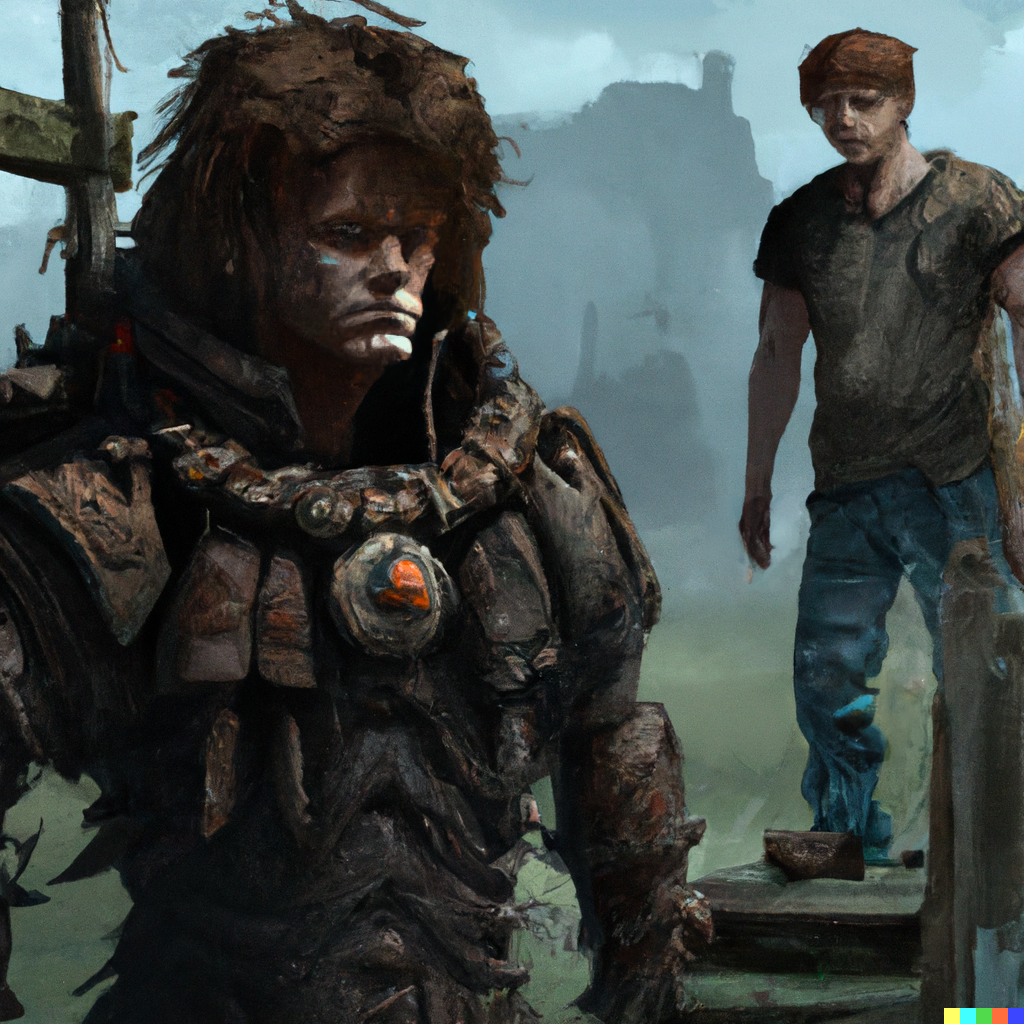
\includegraphics[width=\columnwidth]{characters/character advancement}

    As you accomplish challenges and defeats foes, you gain experience.
    If you have enough experience, you gain a level.
    You gain some abilities at specific levels, as described in \trefnp{Character Advancement}.

    When you gain a level, the following things happen:
    \begin{raggeditemize}
        \item Your \glossterm{hit points} increase (see \pcref{Hit Points}).
        \item Your \glossterm{damage resistance} increases (see \pcref{Damage Resistance}).
        \item You gain an additional \glossterm{archetype rank} (see \pcref{Archetypes})
        \item At even levels, your bonus with \glossterm{trained} skills increases (see \pcref{Trained Skills})
        \item At even levels, your \glossterm{accuracy} increases by 1 (see \pcref{Accuracy})
        \item At even levels, all of your \glossterm{defenses} increase by 1 (see \pcref{Defenses})
        \item At 3rd level, and every 6 levels thereafter, you gain a \glossterm{legacy item} upgrade (see \pcref{Legacy Items}).
        \item At 4th level, and every 3 levels thereafter, your maximum \glossterm{archetype rank} increases (see \pcref{Archetype Ranks}).
    \end{raggeditemize}

    At your GM's discretion, you may also change some of the choices you have made about your character when you level up.
    For example, you could change one of your trained skills for a different skill, change which weapon groups you are proficient with, or change the \glossterm{mystic spheres} you have access to (and corresponding spells).
    The GM may ask for a specific narrative justification for the change, require spending in-game time to retrain, or disallow changing some fundamental aspects of your character.

    \begin{dtable!*}
        \lcaption{Character Advancement}
        \begin{dtabularx}{\textwidth}{l l >{\lcol}X >{\lcol}X l}
            \tb{Level} & \tb{Max Rank}\fn{1} & \tb{Accuracy, Defenses, Skills} & \tb{Special}                        & \tb{XP} \tableheaderrule
            1st        & 1                   & \tdash                          & \tdash                              & 0      \\
            2nd        & \tdash              & \plus1                          & \tdash                              & 10     \\ % +10 xp
            3rd        & \tdash              & \plus1                          & Legacy item: rank 2                 & 25     \\ % +15 xp
            4th        & 2                   & \plus2                          & \tdash                              & 45     \\ % +20 xp
            5th        & \tdash              & \plus2                          & \plus1 \glossterm{attunement point} & 70     \\ % +25 xp
            6th        & \tdash              & \plus3                          & \tdash                              & 100    \\ % +30 xp
            7th        & 3                   & \plus3                          & \tdash                              & 140    \\ % +40 xp
            8th        & \tdash              & \plus4                          & \tdash                              & 200    \\ % +60 xp
            9th        & \tdash              & \plus4                          & Legacy item: ranks 4 and 2          & 300    \\ % +100 xp
            10th       & 4                   & \plus5                          & \tdash                              & 450    \\ % +150 xp
            11th       & \tdash              & \plus5                          & \plus1 \glossterm{attunement point} & 700    \\ % +250 xp
            12th       & \tdash              & \plus6                          & \tdash                              & 1,000  \\ % +300 xp
            13th       & 5                   & \plus6                          & \tdash                              & 1,400  \\ % +400 xp
            14th       & \tdash              & \plus7                          & \tdash                              & 2,000  \\ % +600 xp
            15th       & \tdash              & \plus7                          & Legacy item: ranks 6 and 4          & 3,000  \\ % +1000 xp
            16th       & 6                   & \plus8                          & \tdash                              & 4,500  \\ % +1,500 xp
            17th       & \tdash              & \plus8                          & \tdash                              & 7,000  \\ % +2,500 xp
            18th       & \tdash              & \plus9                          & \tdash                              & 10,000 \\ % +3,000 xp
            19th       & 7                   & \plus9                          & \tdash                              & 14,000 \\
            20th       & \tdash              & \plus10                         & \tdash                              & 20,000 \\
            21st       & \tdash              & \plus10                         & Legacy item: ranks 7 and 6          & 30,000 \\
        \end{dtabularx}
        1. See \pcref{Archetype Ranks}. \\
    \end{dtable!*}

    \subsection{Legacy Items}\label{Legacy Items}

        Over time, items associated with places and people of great power gain magical properties.
        This process takes place for you as you gain levels in addition to in the world as a whole.

        At 3rd level, you choose a nonmagical weapon, body armor, shield, apparel item, or implement you own.
        That item becomes a \glossterm{legacy item}.
        You choose a single magic item property of rank 2 or lower, and your legacy item gains that property.
        You do not have to \glossterm{attune} to your legacy item to gain its benefits.
        However, for each \glossterm{deep attunement} property that your legacy item has, you reduce your maximum \glossterm{attunement points} by one.

        The property must be appropriate for the category of item you chose: weapon, armor, apparel, or implement.
        You do not have to precisely match the location of an apparel item, just the category.
        For example, you can choose an amulet as your legacy item and give it the effect of the \mitem{boots of translocation}, or apply the effects of a \mitem{hardblock shield} to your body armor.

        \parhead{Legacy Item Scaling}
        Your legacy item increases in power as you gain levels.
        At 9th level, you can add an additional item property to your weapon.
        The item property must be rank 4 or lower.
        At 15th and 21st level, you can change the properties on your legacy item, and the maximum rank of both properties increases by 2, to a maximum of rank 7.
        This is summarized below.
        \begin{raggeditemize}
            \item 3rd level character: One property with max rank 2
            \item 9th level character: One property with max rank 4, one property with max rank 2
            \item 15th level character: One property with max rank 6, one property with max rank 4
            \item 21st level character: One properties with max rank 7, one property with max rank 6
        \end{raggeditemize}

        \parhead{Losing Your Legacy Item}
        If you lose your legacy item, you must retrieve it to regain its power.
        There are rituals to facilitate this retrieval such as \ritual{seek legacy} and \ritual{retrieve legacy}.
        If your legacy item is \glossterm{destroyed}, you can designate a new item of the same type to be your legacy item, causing it to gain all of your legacy item abilities.
        Designating a new item in this way requires taking a \glossterm{long rest} while holding or wearing the replacement item.

        \parhead{Unique Legacy Items}
            Legacy items are fundamentally a reflection of the character who wields them.
            Their effects can be more unusual and complex than abilities on normal magic items, and they can have a larger effect on the way that character interacts with the world.
            As a player, you can work with your GM to create custom magical effects of an appropriate power that are a better reflection of your character's personality and powers than the magic item abilities that exist.

\section{Character Statistics}\label{Character Statistics}

    \subsection{Accuracy}\label{Accuracy}
        Your accuracy with an \glossterm{attack} is the number that you add to the \glossterm{attack roll}.
        Your accuracy with an attack is normally equal to half your level \add half your Perception.
        In addition to this base number, your accuracy can include any number of bonuses and penalties from other sources.

    \subsection{Damage Resistance}\label{Damage Resistance}
        Your \glossterm{damage resistance} measures how much damage you can shrug off without any effects.
        For details about how damage resistance is used, see \pcref{Taking Damage}.

        The amount of damage resistance you have is defined in \tref{Hit Points and Damage Resistance}.
        You add your level and your Constitution to find the corresponding base value.
        Body armor also provides a significant bonus to damage resistance, and many special abilities can increase your damage resistance.

        \begin{dtable}
            \lcaption{Hit Points and Damage Resistance}
            \begin{dtabularx}{\columnwidth}{l >{\lcol}X >{\lcol}X}
                \tb{Level \add Con} & \tb{Hit Points} & \tb{Damage Resistance} \tableheaderrule
                0\fn{1}             & 9               & 0  \\
                1                   & 10              & 1  \\
                2                   & 11              & 2  \\
                3                   & 12              & 3  \\
                4                   & 13              & 4  \\
                5                   & 14              & 5  \\
                6                   & 16              & 6  \\
                7                   & 18              & 7  \\
                8                   & 20              & 9  \\
                9                   & 22              & 10 \\
                10                  & 25              & 12 \\
                11                  & 28              & 13 \\
                12                  & 32              & 15 \\
                13                  & 36              & 16 \\
                14                  & 40              & 18 \\
                15                  & 44              & 20 \\
                16                  & 50              & 22 \\
                17                  & 56              & 25 \\
                18                  & 64              & 28 \\
                19                  & 72              & 32 \\
                20                  & 80              & 36 \\
                21                  & 88              & 40 \\
                22\fn{2}            & 100             & 44 \\
            \end{dtabularx}
            1. For negative values, reduce maximum hit points by an amount equal to the negative value. \\
            2. For values beyond 22, double the hit points and damage resistance of a creature with a value that is 6 lower.
            For example, a level 21 creature with a 4 Constitution would have 144 hit points and 64 damage resistance. \\
        \end{dtable}

    \subsection{Defenses}\label{Defenses}
        Usually, when you are attacked, the attacker has to make an \glossterm{attack roll} against one of your four \glossterm{defenses} (see \pcref{Attack Rolls}).
        If the attack roll is at least as high as that defense, the attack hits.
        The four defenses are described below.
        \begin{itemize}
            \item Armor defense (AD): Your Armor defense protects you from normal physical attacks, such as attempts to hit you with a sword.
                It is the most commonly used defense.
            \item Reflex defense: Your Reflex protects you from physical attacks that armor does not help against, such as pit traps or bolts of lightning.
            \item Fortitude defense: Your Fortitude defense protects you from attacks you have to physically endure or resist, such as poisons and life-draining spells.
            \item Mental defense: Your Mental defense protects you from attacks you have to mentally endure or resist, such as terrifying creatures and magical mind manipulation.
        \end{itemize}

        Your defenses are calculated in the following way:
        \begin{itemize}
            \itemhead{Armor} Half level \add Dexterity (modified depending on equipped armor) \add class defense bonus \add defense bonuses from equipped body armor and shield
            \itemhead{Fortitude} Half level \add Constitution \add class defense bonus
            \itemhead{Reflex} Half level \add Dexterity \add class defense bonus
            \itemhead{Mental} Half level \add Willpower \add class defense bonus
        \end{itemize}
        Each defense may also have various bonuses or penalties applied by special abilities.

    \subsection{Encumbrance}\label{Encumbrance}
        Your encumbrance is a value that represents how much you are burdened by your armor (see \pcref{Armor}).
        You apply your encumbrance as a penalty to all Strength and Dexterity-based checks you make.
        If your Strength is positive, you reduce your encumbrance by an amount equal to your Strength.
        This cannot reduce your encumbrance below 0.

    \subsection{Hit Points}\label{Hit Points}
        Your \glossterm{hit points} measure how hard you are to seriously injure or kill.
        For details about how hit points are used, see \pcref{Taking Damage}.

        The amount of hit points you have is defined in \tref{Hit Points and Damage Resistance}.
        You add your level and your Constitution to find the corresponding base value.
        Some special abilities can give you additional \glossterm{hit points}.

        \parhead{What Hit Points Represent} Hit points represent a combination of durability, luck, divine providence, and sheer determination, depending on the nature of the creature being damaged.
        When lose hit points from an orc with a greataxe, the axe did not literally carve into your skin without affecting your ability to fight.
        Instead, you avoided the worst of the blow, but it bruised you through your armor, the effort to dodge the blow fatigued you, or it barely nicked you through sheer luck -- and everyone's luck runs out eventually.

    \subsection{Power}\label{Power}
        Your \glossterm{power} is a general representation of how strong your abilities are.
        Many abilities have stronger effects depending on your \glossterm{power}, especially damaging abilities.
        Your base class provides a bonus to your power (see \pcref{Class-Based Power Bonuses}).
        In addition, some abilities can increase it.

\section{Resources}\label{Resources}

    \subsection{Attunement Points}\label{Attunement Points}
        Many special abilities and magic items only function as long as a creature attunes to them.
        The number of effects that you can attune to is based on the number of \glossterm{attunement points} that you have.
        Most effects require only a single attunement point, but some require two.
        For details, see \pcref{Attunement}.

        Your \glossterm{class} gives you a certain number of attunement points.
        At 5th level and 11th level, you gain an additional attunement point.
        A small number of abilities can also grant additional \glossterm{attunement points}.

    \subsection{Fatigue}\label{Fatigue}
        Thoughout the day, you can become fatigued by your exertions both in and out of combat.
        While \glossterm{hit points} are easy to restore, reducing your \glossterm{fatigue level} generally requires a \glossterm{long rest}.
        Fatigue is still easier to recover from than \glossterm{vital wounds}.

        \subsubsection{Fatigue Level}\label{Fatigue Level}
            Your \glossterm{fatigue level} measures how fatigued you are.
            A number of abilities and attacks can cause you to increase your fatigue level.
            The most common abilities that increase your fatigue level are the \textit{desperate exertion}, \textit{recover}, and \textit{sprint} abilities.
            All of those abilities are described in \pcref{Universal Abilities}.

            \subsubsection{Fatigue Tolerance}\label{Fatigue Tolerance}
                Becoming slightly fatigued is not immediately detrimental.
                Your fatigue level can be as high as your Constitution \add your Willpower without suffering any consequences (minimum 0).
                This value is called your \glossterm{fatigue tolerance}.
                Your \glossterm{class} gives you a bonus to your fatigue tolerance, and some abilities can also modify it.

            \subsubsection{Fatigue Penalty}\label{Fatigue Penalty}
                You take a penalty to \glossterm{accuracy} and \glossterm{checks} equal your \glossterm{fatigue level} \sub your \glossterm{fatigue tolerance}.
                This penalty is called your \glossterm{fatigue penalty}.

        \subsubsection{Exhaustion}\label{Exhaustion}
            When your \glossterm{fatigue penalty} reaches \minus5, you fall \unconscious until your fatigue penalty is reduced below \minus5.
            Generally, this means that you are unconscious for 8 hours.

        \subsubsection{Recovering From Fatigue}
            When you take a \glossterm{long rest}, your \glossterm{fatigue level} is restored to 0 (see \pcref{Resting}).
            There are no other ways to reduce your fatigue level.

\section{Sample Characters}

    This section lists sample characters for each class archetype.
    You can simply pick up one of these characters and use it as your character.
    Alternately, you can use a sample character as a starting point and adjust it to match your own character concept.
    The sample characters are ordered by class first, and by archetype within each class second.

    \subsection{Barbarian}

        \subsubsection{Battleforged Resilience}
            \parhead{Species} Dwarf.
            % 2 1 3 0 2 2 base
            \parhead{Attributes} 2 Str, 0 Dex, 4 Con, 0 Int, 2 Per, 2 Wil (after species modifiers).
            \parhead{Class} Barbarian.
            \parhead{Archetypes} Battleforged Resilience first, Primal Warrior second, Totemist (bear totem) third.
            \parhead{Insight Points} None.
            \parhead{Skills} Awareness, Climb, Endurance, Medicine, Survival
            \parhead{Weapon Groups} Axes, thrown weapons.
            \parhead{Languages} Common, Dwarven, Giantish.
            \parhead{Equipment} Battleaxe, standard shield, scale mail. As you gain levels, use the best medium armor you can afford. If you gain proficiency with heavy armor, use that instead.
            \parhead{Legacy Item} Shield.
                At level 3, choose \mitem{covering shield}.
                At level 9, choose \mitem{greater covering shield} and \mitem{shield of arrow catching}.
                At level 15, choose \mitem{supreme covering shield} and \mitem{greater shield of arrow catching}.
            \parhead{Combat Styles} Herald of War, Unbreakable Defense.
            \parhead{Suggested Feats} Shieldbearer, Martial Training, Regenerator, Toughness.
            \parhead{Combat Tactics} You are extremely difficult to kill.
            Take advantage of that by wading into the front lines of combat and drawing attention away from your more vulnerable allies.
            If you find yourself in danger, use defensive maneuvers like \maneuver{defensive strike} and \maneuver{flamboyant parry} to keep yourself safe.
            On the other hand, if your foes try to ignore you after realizing how durable you are, force them to engage with you using maneuvers like \maneuver{challenging strike} and \maneuver{guard the pass}.

        \subsubsection{Battlerager}
            \parhead{Species} Half-orc.
            % 3 2 2 0 2 1 base
            \parhead{Attributes} 4 Str, 2 Dex, 2 Con, -1 Int, 2 Per, 1 Wil (after species modifiers).
            \parhead{Class} Barbarian.
            \parhead{Archetypes} Battlerager first, Primal Warrior second, Totemist (lion totem) third.
            \parhead{Insight Points} None.
            \parhead{Skills} Awareness, Climb, Endurance, Intimidate, Jump.
            \parhead{Weapon Groups} Crossbows, headed weapons.
            \parhead{Equipment} Greatmace, scale mail. As you gain levels, buy a heavy crossbow and use the best medium armor you can afford.
            \parhead{Legacy Item} Weapon.
                At level 3, choose \mitem{bloodfuel}.
                At level 9, choose \mitem{greater bloodfuel} and \mitem{bloodspray}.
                At level 15, choose \mitem{supreme bloodfuel} and \mitem{greater bloodspray}.
            \parhead{Combat Styles} Ebb and Flow, Herald of War.
            \parhead{Suggested Feats} Greatweapon Warrior, Rapid Reaction, Swiftrunner.
            \parhead{Combat Tactics} You are a furious frenzy of devastating damage and lethal critical hits.
            When you roll a 10 on an attack roll, whatever you attacked will probably die.
            Staying close to your allies is generally a good plan, since you don't have the durability to run into the middle of a horde of enemies safely.
            Your maneuvers help you deal with high-Armor enemies and enemy swarms, and give you the ability to sacrifice most of your statistics other than damage in exchange for more damage.

        \subsubsection{Outland Savage}
            \parhead{Species} Elf.
            % 2 3 2 1 2 0 base
            \parhead{Attributes} 2 Str, 4 Dex, 1 Con, 1 Int, 2 Per, 0 Wil (after species modifiers).
            \parhead{Class} Barbarian.
            \parhead{Archetypes} Outland Savage first, Primal Warrior second, Totemist (wolf totem) third.
            \parhead{Insight Points} 1 point for proficiency with exotic armor weapons.
            \parhead{Skills} Awareness, Climb, Endurance, Jump, Stealth, Survival.
            \parhead{Weapon Groups} Armor weapons, flexible weapons.
            \parhead{Languages} Common, Orcish.
            \parhead{Equipment} Flail, standard shield, scale mail. As you gain levels, use the best light armor you can afford. When you can, get spikes and a spiked knee crafted onto your armor.
            \parhead{Legacy Item} Apparel.
                At level 3, choose \mitem{phasestep boots}.
                At level 9, choose \mitem{enlarging belt} and \mitem{phasestep boots}.
                At level 15, choose \mitem{supreme phasestep boots} and \mitem{enlarging belt}.
            \parhead{Combat Styles} Dirty Fighting, Mobile Assault.
            \parhead{Suggested Feats} Savage, Brawler, Swiftrunner.
            \parhead{Combat Tactics} You can move around the battlefield very quickly, and you are incredibly accurate with special combat actions like shoving and grappling enemies.
            Make the most of that by repositioning enemies, tripping them, or holding them in grapples so your allies can hit them.
            While you aren't in a grapple, use your flail in two hands to maximize your damage.
            When you enter a grapple, use your spiked knee to attack, since your flail is much less effective while grappling.
            If you don't have any allies who like being on the front lines, you won't be as effective at helping them deal damage to enemies, but you're still very skilled at preventing enemies from reaching your allies.
            In that case, consider choosing bear totem or shark totem instead of wolf totem.

        \subsubsection{Primal Warrior}
            \parhead{Species} Human.
            \parhead{Attributes} 3 Str, 2 Dex, 2 Con, 1 Int, 2 Per, 0 Wil.
            \parhead{Class} Barbarian.
            \parhead{Archetypes} Primal Warrior first, Battleforged Resilience second, Outland Savage third.
            \parhead{Insight Points} 1 point for an additional combat style, 1 point for an additional maneuver.
            \parhead{Skills} Awareness, Climb, Endurance, Intimidate, Jump.
            \parhead{Weapon Groups} Axes, crossbows.
            \parhead{Languages} Common, Dwarven, Orcish.
            \parhead{Equipment} Greataxe, scale mail. As you gain levels, buy a heavy crossbow and use the best medium armor you can afford.
            \parhead{Legacy Item} Weapon.
                At level 3, choose \mitem{shocking}.
                At level 9, choose \mitem{banechannel} and \mitem{shocking}.
                At level 15, choose \mitem{greater dimensional trace} and \mitem{banechannel}.
            \parhead{Combat Styles} Dirty Fighting, Herald of War, Unbreakable Defense.
            \parhead{Suggested Feats} Greatweapon Warrior, Weapon Focus, Swiftrunner.
            \parhead{Combat Tactics} You have a great breadth of options available to you thanks to the number of maneuvers you know.
            You have the survivability to stand in close combat, especially if you use maneuvers from Unreakable Defense, but you can also shout at mobile enemies from range with maneuvers from Herald of War.
            Both Dirty Fighting and Herald of War give you maneuvers that work well against enemies with a high Armor defense, so you can adapt to whatever battle you find yourself in.
            You can make the most of your versatility by learning maneuvers like \maneuver{disarm weapon} that are sometimes useless, but which can be devastatingly effective in the right context.

        \subsubsection{Totemist}
            Characters from this archetype can be very different based on their chosen totem.
            A bear totem character might resemble the typical character for the Battleforged Resilience archetype.
            A lion totem or shark totem character might resemble the typical character for the Battlerager archetype.
            A wolf totem character might resemble the typical character for the Outland Savage archetype.

            If you want to quickly create a character based on the eagle totem from this archetype, make the following choices:
            \parhead{Species} Human.
            \parhead{Attributes} 2 Str, 2 Dex, 1 Con, 0 Int, 4 Per, 0 Wil.
            \parhead{Class} Barbarian.
            \parhead{Archetypes} Totemist (eagle totem) first, Primal Warrior second, Outland Savage third.
            \parhead{Insight Points} 1 point for proficiency with exotic bows.
            \parhead{Skills} Awareness, Balance, Climb, Creature Handling, Jump, Survival.
            \parhead{Weapon Groups} Crossbows, bows, thrown weapons.
            \parhead{Languages} Common, Elven, Giantish.
            \parhead{Equipment} Longbow, leather body armor. As you gain levels, buy a flatbow and use the best light armor you can afford.
            \parhead{Legacy Item} Weapon.
                At level 3, choose \mitem{longshot}.
                At level 9, choose \mitem{greater iridescent} and \mitem{longshot}.
                At level 15, choose \mitem{supreme iridescent} and \mitem{greater longshot}.
            \parhead{Combat Styles} Penetrating Precision, Unbreakable Defense.
            \parhead{Suggested Feats} Sniper, Blindfighter, Swiftrunner.
            \parhead{Combat Tactics} You have incredible accuracy from very long range.
            Your defenses are relatively low, but as long as you stay far enough away from your foes, they can't take advantage of that weakness.
            You have the ability to prioritize any target on the battlefield, so make the most of your maneuvers that impose conditions or deal additional damage on weakened foes.

    \subsection{Cleric}

        \subsubsection{Divine Magic}
            \parhead{Species} Gnome.
            % 0 0 2 1 2 4 base
            \parhead{Attributes} -1 Str, 0 Dex, 3 Con, 1 Int, 2 Per, 4 Wil (after species modifiers).
            \parhead{Class} Cleric.
            \parhead{Archetypes} Divine Magic first, Divine Spell Mastery second, Domain Influence third.
            \parhead{Insight Points} 2 points for metamagic (including an extra mystic sphere), and 3 points for additional spells known.
            \parhead{Skills} Knowledge (local, religion), Medicine, Persuasion, Social Insight
            \parhead{Languages} Common, Gnome, Halfling.
            \parhead{Equipment} Mace, standard shield, scale mail. As you gain levels, use the best medium armor you can afford.
            \parhead{Legacy Item} 1-handed implement.
                At level 3, choose \mitem{splitting staff}.
                At level 9, choose \mitem{staff of radiance} and \mitem{splitting staff}.
                At level 15, choose \mitem{greater splitting staff} and \mitem{staff of radiance}.
            \parhead{Domains} Good, Magic
            \parhead{Mystic Spheres} Channel Divinity and Photomancy
            \parhead{Suggested Feats} Celestial Heritage, Sphere Focus: Bless, Sphere Focus: Photomancy
            \parhead{Combat Tactics} You can protect yourself and your allies and invoke divine wrath on your foes.
            Your attacks can hit a variety of defenses, so use the best spells for the situation.
            If you are facing a foe that not particularly vulnerable to your attacks, you can focus on helping your allies with ``boon'' spells to make their actions more effective and keep them safe.

        \subsubsection{Divine Spell Mastery}
            Use the typical character for the Divine Magic cleric archetype.
            Even if you focus on spells through this archetype, you should generally still rank up your spells before improving your rank in this archetype.

        \subsubsection{Domain Influence}
            Characters from this archetype can be very different based on their chosen domains.
            A character with spellcasting-focused domains might resemble the typical character for the Divine Magic cleric archetype.
            If you want to quickly create a more martial character based on the Strength and War domains from this archetype, make the following choices:

            \parhead{Species} Dwarf.
            % 2 1 3 0 2 2 base
            \parhead{Attributes} 2 Str, 0 Dex, 4 Con, 0 Int, 2 Per, 2 Wil (after species modifiers).
            \parhead{Class} Cleric.
            \parhead{Archetypes} Domain Influence first, Divine Magic second, Preacher third.
            \parhead{Insight Points} 3 points for additional spells known.
            \parhead{Skills} Awareness, Knowledge (local, religion), Medicine
            \parhead{Weapon Group} Club-like weapons.
            \parhead{Languages} Common, Draconic, Dwarven.
            \parhead{Equipment} Morning star, standard shield, scale mail. As you gain levels, use the best heavy armor you can afford.
            \parhead{Legacy Item} Armor.
                At level 3, choose \mitem{armor of health}.
                At level 9, choose \mitem{greater armor of health} and \mitem{armor of fortification}.
                At level 15, choose \mitem{supreme armor of health} and \mitem{armor of mystic fortification}, and \mitem{greater featherlight armor}.
            \parhead{Domains} Destruction, War
            \parhead{Mystic Sphere} Channel Divinity
            \parhead{Suggested Feats} Weapon Focus, Sphere Focus: Channel Divinity, Shieldbearer
            \parhead{Combat Tactics} You are a frontline fighter first and foremost.
            Your magically enhanced resistance and high defenses make you durable in combat, though you lack mobility. 
            When you need to distract foes or face down hordes, you can use your abilities from the Preacher archetype.

        \subsubsection{Healer}
            \parhead{Species} Human.
            % 0 2 2 1 0 4 base
            \parhead{Attributes} 0 Str, 2 Dex, 2 Con, 1 Int, 0 Per, 3 Wil.
            \parhead{Class} Cleric.
            \parhead{Archetypes} Healer first, Divine Magic second, Domain Influence third.
            \parhead{Insight Points} 2 points for an additional mystic sphere, 3 points for additional spells known.
            \parhead{Skills} Awareness, Deduction, Knowledge (local, religion), Medicine
            \parhead{Weapon Group} Club-like weapons.
            \parhead{Languages} Common, Draconic, Halfling.
            \parhead{Equipment} Morning star, standard shield, scale mail. As you gain levels, use the best medium armor you can afford.
            \parhead{Legacy Item} 1-handed implement.
                At level 3, choose \mitem{staff of potency}.
                At level 9, choose \mitem{greater staff of potency} and \mitem{staff of pleasant healing}.
                At level 15, choose \mitem{supreme staff of potency} and \mitem{greater staff of pleasant healing}.
            \parhead{Domains} Life, Protection
            \parhead{Mystic Spheres} Bless, Vivimancy
            \parhead{Suggested Feats} Sphere Focus: Vivimancy, Boongiver, Sphere Focus: Bless
            \parhead{Combat Tactics} You have an unmatched mastery of healing and protection.
            You have reasonably high defenses, so you can take to the front lines as necessary to make the most of your \ability{divine aid} and \ability{divine protection} abilities.
            Although your \ability{healer's grace} ability is powerful, you shouldn't feel bad about attacking enemies.
            That's especially important early in a fight when your allies don't need healing yet and your enemies haven't realized that it's pointless to attack your allies while you are still standing.

        \subsubsection{Preacher}
            \parhead{Species} Human.
            \parhead{Attributes} 0 Str, 0 Dex, 2 Con, 2 Int, 4 Per, 0 Wil.
            \parhead{Class} Cleric.
            \parhead{Archetypes} Preacher first, Divine Magic second, Divine Spell Mastery third.
            \parhead{Insight Points} 2 points for metamagic (including an extra mystic sphere), 3 points for additional spells known
            \parhead{Skills} Awareness, Knowledge (local, religion), Linguistics, Medicine, Persuasion, Social Insight
            \parhead{Languages} Common, Dwarven, Elven.
            \parhead{Equipment} Club, standard shield, scale mail. As you gain levels, use the best medium armor you can afford.
            \parhead{Legacy Item} Apparel.
                At level 3, choose \mitem{amulet of blessed oration}.
                At level 9, choose \mitem{greater amulet of blessed oration} and \mitem{greater shieldburst bracers}.
                At level 15, choose \mitem{supreme amulet of blessed oration} and \mitem{supreme shieldburst bracers}.
            \parhead{Mystic Spheres} Enchantment, Revelation
            \parhead{Suggested Feats} Persuasion Specialization, Sphere Focus: Enchantment, Sphere Focus: Revelation
            \parhead{Combat Tactics} Your social skills are virtually unmatched, and you have a wide variety of spells that give you narrative power in social situations.
            In combat, your \ability{denounce the heathens} ability is essentially guaranteed to hit, so you should stay close enough to the front lines to make good use of it.
            You can take advantage of the lowered defenses of your denounced foes to succeed with powerful mind-affecting spells.

    \subsection{Druid}

        \subsubsection{Elementalist}
            \parhead{Species} Human.
            \parhead{Attributes} 0 Str, 0 Dex, 1 Con, 2 Int, 4 Per, 2 Wil.
            \parhead{Class} Druid.
            \parhead{Archetypes} Nature Magic first, Elementalist second, Nature Spell Mastery third.
            \parhead{Insight Points} 2 points for a mystic sphere, 1 point for metamagic (choosing an extra mystic sphere), 3 points for spells
            \parhead{Skills} Awareness, Balance, Jump, Knowledge (dungeoneering, nature), Survival, Swim
            \parhead{Languages} Common, Sylvan
            \parhead{Equipment} Sickle, buckler, hide armor. As you gain levels, keep using hide armor.
            You may want to keep leather armor around in case you need to do a lot of jumping or swimming - or at high levels, flying.
            \parhead{Legacy Item} Implement.
                At level 3, choose \mitem{staff of potency}.
                At level 9, choose \mitem{greater staff of potency} and \mitem{greater selective staff}.
                At level 15, choose \mitem{supreme staff of potency} and \mitem{supreme selective staff}.
            \parhead{Mystic Spheres} Any three of the four elemental mystic spheres.
            Your \textit{elemental spell} ability gives you access to spells from the fourth mystic sphere.
            That means that the specific three mystic spheres you choose mostly just affect which wands you can use and which feats you can take.
            \parhead{Suggested Feats} Sphere Focus: Aeromancy, Aquamancy, Pyromancy, or Terramancy
            \parhead{Combat Tactics} You are a master of all four elements, so you have an immense variety of options available to you - if you choose the right spells.
            You have a very high accuracy thanks to your Perception and a reasonably high power, so your primary role in combat will usually be to deploy the perfect damaging spell or debuff for the situation.
            Your skills and Elementalist abilities give you a lot of narrative power, so stay alert for opportunities to overcome challenges without needing to fight at all.

        \subsubsection{Nature Magic}
            \parhead{Species} Elf.
            % 0 3 1 1 3 2 base
            \parhead{Attributes} 0 Str, 3 Dex, 0 Con, 1 Int, 4 Per, 2 Wil (after species modifiers).
            \parhead{Class} Druid.
            \parhead{Archetypes} Nature Magic first, Nature Spell Mastery second, Elementalist third.
            \parhead{Insight Points} 1 point for metamagic (choosing an extra mystic sphere), 3 points for spells
            \parhead{Skills} Awareness, Creature Handling, Knowledge (nature), Stealth, Survival
            \parhead{Weapon Group} Headed weapons
            \parhead{Languages} Common, Elven, Halfling.
            \parhead{Equipment} Sickle, buckler, leather armor. As you gain levels, use the best light armor you can afford.
            \parhead{Legacy Item} Implement.
                At level 3, choose \mitem{extending staff}.
                At level 9, choose \mitem{bushwalker's staff} and \mitem{extending staff}.
                At level 15, choose \mitem{supreme extending staff} and \mitem{bushwalker's staff}.
            \parhead{Mystic Spheres} Toxicology, Verdamancy
            \parhead{Suggested Feats} Sphere Focus: Verdamancy, Sphere Focus: Aquamancy, Herbalist
            \parhead{Combat Tactics} You are a master of plants and natural magic.
            Your spells excel at constraining and debilitating your foes, especially with poisons.
            Larger foes tend to be resistant to both poisons and movement impediments, so it's a good idea to have Reflex attacks like \spell{ensnaring grasp} and \spell{fire seeds} to deal with them.

        \subsubsection{Nature Spell Mastery}
            Use the typical character for the Nature Magic druid archetype.
            Even if you focus on spells through this archetype, you should generally still rank up your spells before improving your rank in this archetype.

        \subsubsection{Shifter}
            \parhead{Species} Human.
            \parhead{Attributes} 3 Str, 3 Dex, 3 Con, 0 Int, 0 Per, 0 Wil.
            \parhead{Class} Druid.
            \parhead{Archetypes} Shifter first, Nature Magic second, Wildspeaker third.
            \parhead{Insight Points} 1 point for a wild aspect, 3 points for spells
            \parhead{Skills} Awareness, Balance, Climb, Jump, Stealth, Survival
            \parhead{Languages} Common, Sylvan
            \parhead{Equipment} Natural weapon, buckler, chain shirt. As you gain levels, use the best light armor you can afford.
            \parhead{Legacy Item} Armor.
                At level 3, choose \mitem{lifesaver ring}.
                At level 9, choose \mitem{bracers of mighty fists} and \mitem{lifesaver ring}.
                At level 15, choose \mitem{supreme lifesaver ring} and \mitem{bracers of mighty fists}.
            \parhead{Mystic Sphere} Polymorph
            \parhead{Suggested Wild Aspects} Your choice of wild aspects has a significant effect on your capabilities, so choose wild aspects that match your goals.
            The Bear, Viper, and Wolf forms excel at dealing damage in combat.
            The Bull and Constrictor forms improve your ability to take unusual combat actions.
            Other forms can be useful in specific circumstances and out of combat.
            \parhead{Suggested Feats} Sphere Focus: Polymorph, Regenerator, Brawler, Savage
            \parhead{Combat Tactics} You are a lethal blend of claws and teeth.
            You can shift your form to gain the perfect abilities for your current circumstances, and your high physical attributes make you hard to kill and hard to ignore.
            Your flexibility between natural weapons, spells, and high physical skills give you a lot of options in and out of combat.
            In general, you do the most damage in close quarters where you can attack with your natural weapons, but you can use your spells to soften up strong enemies and finish off weakened enemies.

        \subsubsection{Wildspeaker}
            \parhead{Species} Gnome.
            \parhead{Attributes} -1 Str, 0 Dex, 3 Con, 0 Int, 4 Per, 2 Wil.
            \parhead{Class} Druid.
            \parhead{Archetypes} Wildspeaker first, Nature Magic second, Nature Spell Mastery third.
            \parhead{Insight Points} 1 point for metamagic, 3 points for spells.
            \parhead{Skills} Awareness, Creature Handling, Knowledge (nature), Ride, Survival
            \parhead{Weapon Group} Headed weapons
            \parhead{Languages} Common, Gnome, Sylvan
            \parhead{Equipment} Sickle, buckler, scale mail. As you gain levels, use the best medium armor you can afford.
            \parhead{Legacy Item} Apparel.
                At level 3, choose \mitem{amulet of sturdy companionship}.
                At level 9, choose \mitem{greater amulet of sturdy companionship} and \mitem{shrinking belt}.
                At level 15, choose \mitem{supreme amulet of sturdy companionship} and \mitem{greater shrinking belt}.
            \parhead{Mystic Sphere} Electromancy
            \parhead{Suggested Feats} Sphere Focus: Electromancy, Ride Specialization, Creature Handling Specialization, Toughness
            \parhead{Combat Tactics} You lead your faithful natural servant in battle.
            It distracts your enemies while you blast them with lightning from afar.
            Once you get a \textit{shrinking belt} or some other way to shrink yourself, you can ride your \textit{natural servant} into battle, which compensates for your short gnomish legs.
            If you are both lucky and persuasive, you be able to use your \textit{speak with animals} ability to convince an animal to aid you on your journey, at least for a short time, in addition to your \textit{natural servant}.

    \subsection{Fighter}

        \subsubsection{Combat Discipline}
            \parhead{Species} Dwarf.
            % 3 1 3 1 0 2 base
            \parhead{Attributes} 3 Str, 0 Dex, 4 Con, 1 Int, 0 Per, 2 Wil (after species modifiers).
            \parhead{Class} Fighter.
            \parhead{Archetypes} Combat Discipline first, Martial Mastery second, Sentinel third.
            \parhead{Insight Points} 3 points for maneuvers.
            \parhead{Skills} Climb, Endurance, Jump, Swim
            \parhead{Weapon Groups} Axes, crossbows
            \parhead{Languages} Common, Dwarven, Orcish.
            \parhead{Equipment} Battleaxe, standard shield, scale mail. As you gain levels, buy a heavy crossbow and use the best heavy armor you can afford.
            You can switch between a shepherd's axe for hard to hit enemies, a battleaxe for multi-enemy fights or fights where you need the extra damage from holding it in two hands, and throwing axes when you need a ranged weapon.
            \parhead{Legacy Item} Shield.
                At level 3, choose \mitem{shield of arrow catching}.
                At level 9, choose \mitem{hardblock shield} and \mitem{shield of arrow catching}.
                At level 15, choose \mitem{supreme shield of arrow catching} and \mitem{hardblock shield}.
            \parhead{Combat Styles} Rip and Tear, Unbreakable Defense
            \parhead{Suggested Feats} Shieldbearer, Toughness, Regenerator
            \parhead{Combat Tactics} You are extremely difficult to kill, and your ability to ignore and remove conditions makes it hard for your foes to whittle you down over time.
            You can charge confidently into the middle of battle, cutting down enemy ranged attackers regardless of their surrounding allies.
            Alternately, you can hold the line to protect your own allies.

        \subsubsection{Equipment Training}
            \parhead{Species} Halfling.
            % 2 4 1 0 2 0 base
            \parhead{Attributes} 1 Str, 5 Dex, 0 Con, 1 Int, 2 Per, 0 Wil.
            \parhead{Class} Fighter.
            \parhead{Archetypes} Equipment Training first, Martial Mastery second, Combat Discipline third.
            \parhead{Insight Points} 3 points for maneuvers.
            \parhead{Skills} Awareness, Balance, Flexibility, Stealth
            \parhead{Weapon Groups} Blades, bows
            \parhead{Languages} Common, Gnomish, Halfling
            \parhead{Equipment} Kukri, standard shield, scale mail. As you gain levels, buy a longbow and use the best armor you can afford that allows you to apply your full Dexterity bonus to your Armor defense.
                Keep an extra kukri with you so you can dual wield in fights where you don't need to use a shield.
            \parhead{Legacy Item} Weapon.
                At level 3, choose \mitem{potency}.
                At level 9, choose \mitem{greater potency} and \mitem{seeking}.
                At level 15, choose \mitem{supreme potency} and \mitem{wolfpack}.
            \parhead{Combat Styles} Flurry of Blows, Rip and Tear
            \parhead{Suggested Feats} Swiftrunner, Rapid Reaction, Executioner, Two-Weapon Fighting
            \parhead{Combat Tactics} You have an exceptionally high Armor defense, and your strikes are very accurate.
            However, your low Strength and small weapons mean that you don't deal a lot of damage.
            Focus on debilitating maneuvers like \maneuver{brow gash} or maneuvers that increase your damage like \maneuver{tear exposed flesh} to stay relevant in combat.
            When your Armor defense isn't as important, such as when fighting spellcasters, you can dual wield to increase your damage.
            Unlike most fighters, you are very agile and stealthy, so you can accompany rogues on scouting missions.

        \subsubsection{Martial Mastery}
            \parhead{Species} Human.
            \parhead{Attributes} 4 Str, 0 Dex, 2 Con, 1 Int, 2 Per, 0 Wil.
            \parhead{Class} Fighter.
            \parhead{Archetypes} Martial Mastery first, Combat Discipline second, Tactician third.
            \parhead{Insight Points} 1 point for an additional combat style, 3 points for maneuvers.
            \parhead{Skills} Awareness, Climb, Endurance, Jump, Swim
            \parhead{Weapon Groups} Blades, thrown weapons.
            \parhead{Languages} Common, Giantish, Orcish.
            \parhead{Equipment} Broadsword, standard shield, scale mail. As you gain levels, buy throwing axes and use the best heavy armor you can afford.
            \parhead{Legacy Item} Armor.
                At level 3, choose \mitem{resistant armor}.
                At level 9, choose \mitem{greater resistant armor} and \mitem{armor of fortification}.
                At level 15, choose \mitem{supreme resistant armor} and \mitem{armor of mystic fortification}.
            \parhead{Combat Styles} Ebb and Flow, Herald of War, Rip and Tear
            \parhead{Suggested Feats} Executioner, Blindfighter, Toughness
            \parhead{Combat Tactics} You have great versatility in combat.
            You have a large number of manuvers, and by mixing in thrown weapons and shouts, you can attack at multiple ranges and hit multiple defenses.
            When your shield is unnecessary, you can hold your broadsword in two hands to improve your already respectable damage.
            Many of your maneuvers work at any range, so you aren't forced to fight in melee against highly mobile or excessively lethal foes.
            In addition to using maneuvers, you can coordinate your allies with battle tactics.

        \subsubsection{Sentinel}
            \parhead{Species} Dwarf.
            % 2 1 2 0 4 0 base
            \parhead{Attributes} 2 Str, 0 Dex, 3 Con, 0 Int, 4 Per, 0 Wil.
            \parhead{Class} Fighter.
            \parhead{Archetypes} Sentinel first, Martial Mastery second, Equipment Training third.
            \parhead{Insight Points} 2 points for maneuvers.
            \parhead{Skills} Awareness, Endurance, Intimidate
            \parhead{Weapon Groups} Axes, crossbows
            \parhead{Languages} Common, Dwarven, Orcish
            \parhead{Equipment} Shepherd's axe, standard shield, scale mail. As you gain levels, buy a throwing axes, a heavy crossbow, and a greataxe and use the best heavy armor you can afford.
            \parhead{Legacy Item} Apparel.
                At level 3, choose \mitem{protector's amulet}.
                At level 9, choose \mitem{greater boots of speed} and \mitem{protector's amulet}.
                At level 15, choose \mitem{supreme boots of speed} and \mitem{greater protector's amulet}.
            \parhead{Combat Styles} Rip and Tear, Unbreakable Defense
            \parhead{Suggested Feats} Shieldbearer, Toughness, Regenerator
            \parhead{Combat Tactics} You hold the line in the middle of the fray, protecting your allies all over the battlefield.
            You have an unmatched ability to constrain your foes' movement and force them to pay attention to you, limiting their ability to harm your allies.
            Your damage is reasonable, but your main focus should be on defense so you can protect your more vulnerable and reckless allies.
            A shepherd's axe is convenient because it allows you to attack foes who try to keep their distance from you.
            However, when you need to deal damage, consider switching to a greataxe or dual-wielding a second shepherd's axe instead of holding a shield.

        \subsubsection{Tactician}
            \parhead{Species} Human.
            \parhead{Attributes} 2 Str, 3 Dex, 1 Con, 2 Int, 2 Per, 0 Wil.
            \parhead{Class} Fighter.
            \parhead{Archetypes} Tactician first, Martial Mastery second, Equipment Training third.
            \parhead{Insight Points} 2 points for battle tactics, 3 points for maneuvers.
            % 3 fighter + 2 int + 1 human = 6 trained
            \parhead{Skills} Awareness, Deduction, Endurance, Knowledge (dungeoneering, local), Medicine
            \parhead{Weapon Groups} Bows, polearms.
            \parhead{Languages} Common, Draconic, Elven
            \parhead{Equipment} Longhammer, standard shield, chain shirt. As you gain levels, buy a longbow and use the best armor you can afford that allows you to apply your full Dexterity bonus to your Armor defense.
            \parhead{Legacy Item} Weapon.
                At level 3, choose \mitem{resistant armor}.
                At level 9, choose \mitem{greater resistant armor} and \mitem{swiftstep armor}.
                At level 15, choose \mitem{supreme resistant armor}, \mitem{greater swiftstep armor}, and \mitem{greater armor of health}.
            \parhead{Combat Styles} Blunt Force, Mobile Assault
            \parhead{Suggested Feats} Precognition, Leadership, Medicine Specialization
            \parhead{Combat Tactics} You have a wealth of options in combat.
            You can buff your allies' attacks, defend your allies, deal damage, or debuff your foes.
            Use whichever battle tactics are most relevant to the current situation.
            Your longhammer and high mobility allows you to keep your distance in combat while knocking your foes into more tactically advantageous positions.
            Since you don't use a shield, you don't have the defensive power of most fighters, so you can't just charge heedlessly into the fray.

    \subsection{Monk}

        \subsubsection{Airdancer}
            \parhead{Species} Elf.
            % Base 2 4 1 0 2 0
            \parhead{Attributes} 2 Str, 5 Dex, 0 Con, 0 Int, 2 Per, 0 Wil.
            \parhead{Class} Monk.
            \parhead{Archetypes} Airdancer first, Esoteric Warrior second, Ki third.
            \parhead{Insight Points} 1 point for a ki manifestation, 1 point for a maneuver.
            \parhead{Skills} Balance, Climb, Flexibility, Jump, Stealth, Swim
            \parhead{Weapon Groups} Monk weapons
            \parhead{Languages} Common, Elven, Halfling
            \parhead{Equipment} Two jitte. Use your \textit{ki barrier} for your body armor.
            \parhead{Legacy Item} Apparel.
                At level 3, choose \mitem{boots of levitation}.
                At level 9, choose \mitem{greater boots of levitation} and \mitem{greater boots of reliable motion}.
                At level 15, choose \mitem{supreme boots of levitation} and \mitem{supreme boots of reliable motion}.
            \parhead{Combat Styles} Mobile Assault, Penetrating Precision
            \parhead{Suggested Feats} Jump Specialization, Balance Specialization, Swiftrunner, Two-Weapon Fighting
            \parhead{Combat Tactics} You are highly acrobatic in combat, leaping around your opponents with ease.
            Once your Jump check result is high enough to jump over enemies, you can start ignoring attempts to block your movement.
            The Leap of the Heavens \textit{ki manifestation} can help you reach that point quickly.
            You are highly accurate, and your high Dexterity helps both your defenses and your skills.
            If you are in physical danger, you can sheathe one of your kamas and use your \textit{ki barrier} as a shield to further increase your Armor defense.
            However, your middling Constitution means you should pick your fights carefully.
            Use your mobility to pick your battles and avoid being surrounded unnecessarily.

        \subsubsection{Esoteric Warrior}
            \parhead{Species} Human
            \parhead{Attributes} 2 Str, 3 Dex, 2 Con, 1 Int, 2 Per, 0 Wil.
            \parhead{Class} Monk.
            \parhead{Archetypes} Esoteric Warrior first, Perfected Form second, Transcendent Sage third.
            \parhead{Insight Points} 4 points for maneuvers.
            \parhead{Skills} Awareness, Balance, Climb, Flexibility, Endurance, Medicine, Jump, Stealth
            \parhead{Weapon Groups} Monk weapons
            \parhead{Languages} Common, Draconic, Elven
            \parhead{Equipment} Two kunai, chain shirt. As you gain levels, buy spare kunai, and use the best light armor you can afford.
            \parhead{Legacy Item} Apparel.
                At level 3, choose \mitem{gauntlet of the ram}.
                At level 9, choose \mitem{bracers of mighty fists} and \mitem{boots of speed}.
                At level 15, choose \mitem{supreme boots of speed} and \mitem{bracers of mighty fists}.
            \parhead{Combat Styles} Dirty Fighting, Flurry of Blows
            \parhead{Suggested Feats} Brawler, Juggernaut, Swiftrunner, Two-Weapon Fighting
            \parhead{Combat Tactics} You can beat your opponents to death with nothing more than your bare hands.
            Your primary combat strategy is generally to grapple, trip, or otherwise debuff your opponents with your free hands before you pummel them into submission.
            You have a high movement speed, and you can take advantage of that by rushing down enemies who would prefer to keep their distance.
            When that is combined with your immunity to many common debuffs, you are exceptionally effective against enemy spellcasters.
            If you find yourself fighting more martially skilled foes, you may need to keep your distance with kunai or a bow, at least until they are weakened.

        \subsubsection{Ki}
            \parhead{Species} Halfling
            % 0 2 2 1 0 4 base
            \parhead{Attributes} -1 Str, 2 Dex, 2 Con, 1 Int, 0 Per, 5 Wil.
            \parhead{Class} Monk.
            \parhead{Archetypes} Ki first, Esoteric Warrior second, Transcendent Sage third.
            \parhead{Insight Points} 2 points for ki manifestations, 1 point for a maneuver.
            \parhead{Skills} Balance, Flexibility, Endurance, Medicine, Knowledge (arcana), Survival, Stealth
            \parhead{Weapon Groups} Monk weapons
            \parhead{Languages} Common, Draconic, Elven
            \parhead{Equipment} Two kama. Use your \textit{ki barrier} for your body armor. As you gain levels, buy spare kunai.
            \parhead{Legacy Item} Weapon.
                At level 3, choose \mitem{potency}.
                At level 9, choose \mitem{greater potency} and \mitem{hefty}.
                At level 15, choose \mitem{supreme potency} and \mitem{greater hefty}
            \parhead{Combat Styles} Flurry of Blows, Mobile Assault
            \parhead{Suggested Feats} Two-Weapon Fighting, Ghostblade, Iron Will, Spellwarped
            \parhead{Combat Tactics} Although you appear small and physically weak, your attacks hit hard thanks to your \textit{ki energy} ability.
            You can use a variety of ki manifestations to have surprising effects in combat.
            Look for tricky combinations, like tripping your foes at a distance with \ability{extend the flow of ki} or using \ability{burst of blinding speed} to increase the power of movement-based maneuvers.
            You can also use your ki manifestations to augment your skills in non-combat situations.
            Your defenses are high and well-rounded, and you have immunities to a variety of common debuffs, so you can fight aggressively in combat.
            Generally, you should dual-wield kama, but you can drop to a single kama if you need more Armor defense, or you can switch to throwing kunai to hit distant foes.

        \subsubsection{Perfected Form}
            \parhead{Species} Human
            \parhead{Attributes} 3 Str, 3 Dex, 3 Con, 0 Int, 0 Per, 0 Wil.
            \parhead{Class} Monk.
            \parhead{Archetypes} Perfected Form first, Esoteric Warrior second, Airdancer third.
            \parhead{Insight Points} 1 point for a trained skill, 2 points for maneuvers.
            \parhead{Skills} Balance, Climb, Flexibility, Endurance, Jump, Stealth, Swim
            \parhead{Weapon Groups} Monk weapons
            \parhead{Languages} Common, Giantish, Orcish
            \parhead{Equipment} Two kunai, chain shirt. As you gain levels, buy spare kunai, and use the best light armor you can afford.
            \parhead{Legacy Item} Apparel.
                At level 3, choose \mitem{gauntlet of the ram}.
                At level 9, choose \mitem{bracers of mighty fists} and \mitem{boots of speed}.
                At level 15, choose \mitem{supreme boots of speed} and \mitem{bracers of mighty fists}.
            \parhead{Combat Styles} Dirty Fighting, Mobile Assault
            \parhead{Suggested Feats} Brawler, Juggernaut, Swiftrunner, Two-Weapon Fighting
            \parhead{Combat Tactics} Your general fighting style is the same as the Esoteric Warrior sample character.
            Your main differentiating factor is that you have even greater martial aptitude and durability.
            However, you are less able to avoid to debilitating conditions, so be careful when fighting magical foes.

        \subsubsection{Transcendent Sage}
            The transcendent sage archetype by itself does not strongly influence your character's fighting style or abilities.
            It provides a variety of passive abilities and immunities that require other archetypes to make a compelling character concept.
            A typical character focusing on this archetype would be similar to the Ki character.
            If you want to be more martially inclined, follow the Esoteric Warrior character.

    \subsection{Paladin}

        \subsubsection{Devoted Paragon}
            The devoted paragon archetype can have different play styles based on your devoted alignment.
            The character below is reasonable for any alignment other than evil.
            An evil devoted paragon might focus more on inflicting debilitating conditions with spells from the \sphere{enchantment} or \sphere{vivimancy} \glossterm{mystic spheres}.

            \parhead{Species} Dwarf
            % 2 1 3 2 0 2
            \parhead{Attributes} 2 Str, 0 Dex, 4 Con, 0 Int, 2 Per, 2 Wil.
            \parhead{Class} Paladin.
            \parhead{Archetypes} Devoted Paragon first, Divine Magic second, Stalwart Guardian third.
            \parhead{Insight Points} 2 points for spells.
            \parhead{Skills} Endurance, Persuasion, Social Insight
            \parhead{Weapon Groups} Club-like weapons, crossbows.
            \parhead{Languages} Common, Dwarven, Giantish
            \parhead{Equipment} Morning star, standard shield, scale mail. As you gain levels, buy a heavy crossbow and use the best heavy armor you can afford.
            \parhead{Legacy Item} Shield.
                At level 3, choose \mitem{covering shield}.
                At level 9, choose \mitem{greater covering shield} and \mitem{soulguard shield}.
                At level 15, choose \mitem{shield of mystic reflection} and \mitem{greater covering shield}.
            \parhead{Mystic Sphere} Bless.
            \parhead{Suggested Feats} Leadership, Weapon Focus, Shieldbearer, Sphere Focus: Bless
            \parhead{Combat Tactics} You are a beacon to guide your allies in combat.
            You should stay close to the front lines to ensure that your allies gain the benefit of your \textit{aligned aura} ability and take advantage of your reasonable melee damage.
            You are very durable, and you can blanket your allies with powerful buffs from the \sphere{bless} mystic sphere.
            At high levels, make sure you have a special strike ability like \spell{exalted strike} or a \mitem{powerstrike} weapon.

        \subsubsection{Divine Magic}

            \parhead{Species} Human
            \parhead{Attributes} 1 Str, 0 Dex, 2 Con, 2 Int, 0 Per, 4 Wil.
            \parhead{Class} Paladin.
            \parhead{Archetypes} Divine Magic first, Divine Spell Expertise second, Devoted Paragon third.
            \parhead{Insight Points} 2 points for an extra mystic sphere, 3 points for spells.
            \parhead{Skills} Endurance, Medicine, Persuasion
            \parhead{Weapon Groups} Axes, thrown weapons.
            \parhead{Languages} Common, Dwarven, Giantish
            \parhead{Equipment} Battleaxe, standard shield, scale mail. As you gain levels, use the best heavy armor you can afford and switch to using an implement instead of a weapon.
            \parhead{Legacy Item} Implement.
                At level 3, choose \mitem{potency}.
                At level 9, choose \mitem{greater covering shield} and \mitem{soulguard shield}.
                At level 15, choose \mitem{shield of mystic reflection} and \mitem{greater covering shield}.
            \parhead{Mystic Sphere} Channel Divinity, Vivimancy.
            \parhead{Suggested Feats} Sphere Focus: Channel Divinity, Sphere Focus: Vivimancy, Boongiver
            \parhead{Combat Tactics} Paladins make unusual spellcasters.
            They lack the flexibility of more dedicated spellcasting classes because they lack the \ability{metamagic} ability and access to a variety of mystic spheres.
            However, your \textit{divine spell versatility} and \textit{divine conduit} give you a unique combat style that rewards staying directly on the front lines.
            In addition, you have an unusually high power thanks to \textit{wellspring of power} and \textit{paragon power}, so your damage and healing spells can be quite potent.
            Make sure you have single-target damage spells like \spell{mystic bolt} and \spell{lifesteal} to make the most of your abilities.

        \subsubsection{Divine Spell Expertise}
            Use the typical character for the Divine Magic paladin archetype.
            Even if you focus on spells through this archetype, you should generally still rank up your spells before improving your rank in this archetype.

        \subsubsection{Stalwart Guardian}

            \parhead{Species} Halfling
            % 0 3 3 0 0 3 base
            \parhead{Attributes} -1 Str, 3 Dex, 3 Con, 0 Int, 0 Per, 4 Wil (after species modifiers).
            \parhead{Class} Paladin.
            \parhead{Archetypes} Stalwart Guardian first, Divine Magic second, Zealous Warrior third.
            \parhead{Insight Points} 2 points for spells.
            \parhead{Skills} Endurance, Medicine, Ride
            \parhead{Weapon Groups} Club-like weapons, thrown weapons.
            \parhead{Languages} Common, Dwarven, Giantish
            \parhead{Equipment} Smallsword, standard shield, scale mail. As you gain levels, buy spare throwing axes and use the best light armor you can afford.
            \parhead{Legacy Item} Apparel.
                At level 3, choose \mitem{amulet of divine healing}.
                At level 9, choose \mitem{greater amulet of divine healing} and \mitem{boots of speed}.
                At level 15, choose \mitem{supreme amulet of divine healing} and \mitem{greater boots of speed}.
            \parhead{Mystic Sphere} Fabrication.
            \parhead{Suggested Feats} Shieldbearer, Sphere Focus: Bless
            \parhead{Combat Tactics} You have exceptionally high defenses, and you can heal your less well protected allies.
            Your damage is reasonable thanks to your \ability{smite} ability, which allows you to use your high Willpower in place of your poor Strength.
            You can use spells like \spell{mystic barrier} and \spell{blade barrier} to control the battlefield and funnel your foes into positions where you can make the most of your defensive abilities.

        \subsubsection{Zealous Warrior}

            \parhead{Species} Elf
            % 1 0 1 0 3 4 base
            \parhead{Attributes} 1 Str, 0 Dex, 0 Con, 0 Int, 4 Per, 4 Wil (after species modifiers).
            \parhead{Class} Paladin.
            \parhead{Archetypes} Zealous Warrior first, Divine Magic second, Stalwart Guardian third.
            \parhead{Insight Points} 2 points for spells.
            \parhead{Skills} Awareness, Persuasion, Social Insight
            \parhead{Weapon Groups} Club-like weapons, bows
            \parhead{Languages} Common, Dwarven, Giantish
            \parhead{Equipment} Greatmace, scale mail. As you gain levels, buy a longbow and use the best heavy armor you can afford.
            \parhead{Legacy Item} Weapon.
                At level 3, choose \mitem{potency}.
                At level 9, choose \mitem{greater potency} and \mitem{blessed}.
                At level 15, choose \mitem{supreme potency} and \mitem{honed}.
            \parhead{Mystic Sphere} Channel Divinity.
            \parhead{Suggested Feats} Greatweapon Warrior, Spellsword, Celestial Heritage
            \parhead{Combat Tactics} You are an extremely dangerous martial combatant.
            Thanks to your \ability{smite} ability, you have high damage and devastatingly powerful critical hits.
            Your defenses are unimpressive, but you have enough damage resistance from heavy armor to avoid being too squishy.
            The biggest weakness you have is your slow speed and vulnerability to debilitating conditions.
            Make sure you take some ranged spells like \spell{retributive judgment} to deal with foes who try to avoid your greatmace.

            Alternately, you could focus more heavily on ranged combat, since \ability{smite} can be used with projectile weapons.
            If that is your goal, consider the Mystic Archer and Sniper feats instead of Greatweapon Warrior and Spellsword.
